\chapterOrPart{Methodology}\label{ch:materialsmethods}

\section{Methodological Scope}
\label{sec:methodological_scope}
 
The objective of this work is to quantify how Belgian residential energy demand may evolve under changing climate forcing and changing household technology stocks, while preserving household-level behavioural variability. This requires a model that resolves dwellings and end-uses, responds physically to weather, and keeps climate, technology, and stochastic variation separable in the results.\footnote{Throughout this section, the modelling paradigm is positioned against the residential demand modelling literature surveyed by \textcite{swan_modeling_2009,kavgicReviewBottomupBuilding2010, Allegrini2015}.} \Cref{fig:scope_taxonomy} situates the chosen paradigm against the broader taxonomy of residential demand models.
 
% ---------------------------------------------------------------------
% Figure: taxonomy of residential demand models with our position
% ---------------------------------------------------------------------
\begin{figure}[ht]
  \centering
  \begin{tikzpicture}[
      every node/.style={font=\footnotesize, align=center},
      box/.style={draw, rounded corners=2pt, inner sep=4pt,
                  minimum height=9mm, minimum width=22mm},
      pick/.style={box, fill=black!8, very thick},
      arrow/.style={-{Latex[length=2mm]}, semithick},
      node distance=10mm and 14mm,
  ]
    % Column 1: root
    \node[box] (root) {Residential\\energy demand\\models};
 
    % Column 2: top-down / bottom-up (stacked vertically)
    \node[box, above right=4mm and 14mm of root] (td) {Top-down};
    \node[box, below right=4mm and 14mm of root] (bu) {Bottom-up};
    \draw[arrow] (root.east) -- (td.west);
    \draw[arrow] (root.east) -- (bu.west);
 
    % Column 3: leaf families
    \node[box, right=14mm of td, fill=black!3]
      (td_ex) {Econometric,\\regression};
    \node[box, above right=2mm and 14mm of bu]  (stat) {Statistical\\(data-driven)};
    \node[box, below right=2mm and 14mm of bu]  (eng)  {Engineering\\(physics-based)};
    \draw[arrow, dotted] (td.east) -- (td_ex.west);
    \draw[arrow] (bu.east) -- (stat.west);
    \draw[arrow] (bu.east) -- (eng.west);
 
    % Column 4: hybrid pick (vertically centred between stat and eng)
    \node[pick, right=14mm of bu, xshift=32mm]
      (hyb) {\textbf{Hybrid}\\stochastic +\\physics-informed};
    \draw[arrow, dashed] (stat.east) -- (hyb.west);
    \draw[arrow, dashed] (eng.east)  -- (hyb.west);
  \end{tikzpicture}
  \caption{Position of the proposed model within the residential demand modelling taxonomy.}
  \label{fig:scope_taxonomy}
\end{figure}
The model is bottom-up (per-dwelling, per-end-use) and combines a stochastic occupancy/behaviour layer with a physics-informed thermal and technology layer, following the hybrid family introduced by \textcite{Capasso1994,Richardson2010_DomesticHighRes,McKenna2015}. A bottom-up formulation is required because the thesis compares technology substitution, weather sensitivity, and cohort peak coincidence rather than only aggregate annual demand.


\subsection{Hybrid Approach}
\label{sec:hybrid_approach}
 
This work adopts a hybrid formulation in the sense of \textcite{Capasso1994}, refined by the CREST family of models \cite{Richardson2010CRESTElectricity,McKenna2015} and the behavioural-physics couplings reviewed by \textcite{Sandels2016,DOca2017}. Concretely:
\begin{itemize}[leftmargin=1.2em, itemsep=2pt, topsep=2pt]
  \item Stochasticity is introduced at the \emph{behavioural} layer, through a probabilistic occupancy and activity model that drives the metabolic, lighting, appliance, cooking, and DHW end-uses. This recovers between-household diversity, plausible coincidence factors, and load-shape variability without prescribing a single average profile.
  \item Physics is introduced at the \emph{thermal} and \emph{system} layers, through a reduced-order (lumped-capacitance) building thermal balance and through temperature-dependent conversion efficiencies. This guarantees that space heating and electrified heating respond mechanistically to outdoor temperature and solar gains, which is the channel through which \hyperref[sec:climateScenariosFramework]{climate scenarios} act.
\end{itemize}
 
This combination is the minimum modelling content required for the research question: weather sensitivity comes from the physical layers, while diversity and coincidence come from the stochastic layers.


\subsection{Base Framework}
\label{sec:base_framework}
 
The resulting framework is therefore a \emph{stochastic, physics-informed, bottom-up} model of residential energy demand. Its data contract follows the canonical pipeline used in the model implementation:
 
\begin{equation}\label{eq:dataContract}
\begin{split}
  \underbrace{\text{InputDataset}}_{\text{dwelling, weather, tech}}
  &\to
  \underbrace{\text{PreparedForcing}}_{\text{time-aligned drivers}}
  \to
  \underbrace{\text{PhysicsState}}_{\text{thermal balance}}\\
  &\to
  \underbrace{\text{ControlState}}_{\text{thermostat, deadband}}
  \to
  \underbrace{\text{SystemState}}_{\text{carriers, PV, EV, grid}}
  \to
  \underbrace{\text{ModelOutputs}}_{\text{kWh, kW, HDD, etc.}}
\end{split}
\end{equation}
 
Each block is a typed interface, so the boundary between behaviour, physics, control, and systems remains auditable. The same pipeline is reused across deterministic annual runs, stochastic cohort simulations, and scenario-tree experiments; only the configuration changes.


\subsection{System Boundary}
\label{sec:system_boundary}
 
A defensible scope requires an explicit boundary. \Cref{fig:system_boundary} summarises the boundary adopted in this work: climate forcing and technology assumptions enter as exogenous inputs; behaviour, physics, control, and systems are simulated endogenously; and the outputs are final energy per carrier, peak power, grid exchange, and comfort indicators.
 
% ---------------------------------------------------------------------
% Figure: explicit system boundary
% ---------------------------------------------------------------------
\begin{figure}[ht]
  \centering
  % \resizebox scales the whole picture (including its text) to \textwidth
  % so the diagram can never overflow horizontally.
  \resizebox{\textwidth}{!}{%
  \begin{tikzpicture}[
      every node/.style={font=\footnotesize, align=center},
      block/.style={draw, rounded corners=2pt, inner sep=3pt,
                    minimum height=8mm, minimum width=22mm},
      forcing/.style={block, fill=black!3},
      outblock/.style={block, fill=black!8},
      arrow/.style={-{Latex[length=2mm]}, semithick},
      node distance=6mm and 8mm,
  ]
    % --- Inside the boundary (placed first, boundary fits around them) ---
    \node[block]                    (ctrl) {Control};
    \node[block, right=of ctrl]     (phys) {Thermal balance};
    \node[block, right=of phys]     (sys)  {Energy systems};
    \node[block, above=5mm of phys] (occ)  {Occupancy \&\\ stochastic activity};
 
    \draw[arrow] (occ)  -- (phys);
    \draw[arrow] (ctrl) -- (phys);
    \draw[arrow] (phys) -- (sys);
 
    % --- Boundary box drawn AROUND the inner nodes via the `fit' library ---
    \node[draw, dashed, rounded corners=4pt, inner sep=5mm,
          fit=(occ)(ctrl)(phys)(sys)] (bnd) {};
    \node[anchor=south west, font=\footnotesize\itshape, inner sep=2pt,
          fill=white]
      at ([xshift=3mm,yshift=-0.4mm]bnd.north west)
      {\,System boundary: residential dwelling cohort\,};
 
    % --- Exogenous forcing (left, outside boundary) ---
    \node[forcing, left=10mm of ctrl]            (clim) {Climate forcing\\($T_{\text{out}}$, $G_{\text{sol}}$)};
    \node[forcing, below=3mm of clim, anchor=north west, xshift=0mm]
                                                 (tech) {Technology case};
    \draw[arrow] (clim.east) -- (ctrl.west);
    \draw[arrow] (tech.east) -| ([xshift=-3mm]sys.west) -- (sys.west);
 
    % --- Outputs (right, outside boundary) ---
    \node[outblock, right=10mm of sys] (kWh) {Final energy};
    \node[outblock, above=3mm of kWh]  (com) {Comfort \&\\overheating};
    \node[outblock, below=3mm of kWh]  (kW)  {Peak power\\\& grid exchange};
    \draw[arrow] (sys.east) -- (kWh.west);
    \draw[arrow] (sys.east) -- (com.west);
    \draw[arrow] (sys.east) -- (kW.west);
  \end{tikzpicture}}
  \caption{System boundary of the model.}
  \label{fig:system_boundary}
\end{figure}
 
The scope is the Belgian residential stock, represented through dwelling archetypes and household cohorts. Tertiary, industrial, and transport-sector loads are excluded; EVs enter only as residential charging at the dwelling meter. The model is non-spatial in the network sense, with all dwellings connected to one import/export boundary and climate forcing taken at the Uccle/Brussels reference point. Historical-weather runs use the hourly canonical configuration, while processed CORDEX leaves use their active forcing timestep. Final energy is reported for electricity, natural gas, fuel oil, and other configured heating carriers; primary-energy, emissions, and economic accounting are post-processing layers rather than simulator state.

 
% ---------------------------------------------------------------------
% Table: inclusions / exclusions
% ---------------------------------------------------------------------
\begin{table}[ht]
  \centering
  \footnotesize
  \caption{System boundary: explicit inclusions and exclusions.}
  \label{tab:scope_inclusions_exclusions}
  \begin{tabular}{@{}p{0.46\linewidth} p{0.46\linewidth}@{}}
    \toprule
    \textbf{Inside the boundary} & \textbf{Outside the boundary} \\
    \midrule
    Residential dwellings (per-archetype) &
      Tertiary, industrial, and transport sectors \\
    Stochastic occupancy and activity &
      Detailed agent-based household behaviour \\
    Reduced-order thermal balance &
      Multi-zone CFD or full building-physics simulation \\
    Temperature-dependent heat-pump COPs and conversion losses &
      Component-level HVAC dynamics, refrigerant cycles \\
    PV self-consumption and grid import/export at the dwelling meter &
      Distribution-network impedances, voltage, congestion \\
    Final-energy demand per carrier (electricity, gas, oil) &
      Primary energy, $\mathrm{CO_2}$ accounting \\
    Comfort and overheating indicators (CDD, exceedance hours) &
      Active cooling final-energy consumption \\
    Climate forcing via CORDEX RCP pathways &
      Probabilistic climate forecasts; ensemble downscaling beyond
      the configured GCM/RCM chain \\
    \bottomrule
  \end{tabular}
\end{table}


\subsection{Core Assumptions}
\label{sec:core_assumptions}
 
The load-bearing assumptions of the methodological scope are:
 
\begin{enumerate}[label=A\arabic*., leftmargin=2.2em, itemsep=2pt, topsep=2pt]
  \item \textbf{Single-zone thermal representation.} Each dwelling is modelled as one thermal zone with a lumped UA and thermal mass, consistent with reduced-order residential demand models \cite{Reynders2014_ModelComplexity,Bacher2011}. Inter-room dynamics, stack effects, and humidity are not resolved.
 
  \item \textbf{Independent households.} Households are conditionally
  independent given climate forcing and the technology case; there is no peer-effect or social-network coupling between dwellings. Cohort coincidence emerges from shared exogenous forcing and from the archetype/behaviour distributions.
 
  \item \textbf{No active cooling final energy.} Active cooling is not converted into electricity consumption; cooling pressure is reported only through CDD, indoor overheating hours, and excess-heat indicators.
 
  \item \textbf{No network constraints.} Voltage, congestion, and distribution losses are not modelled. Grid import and export are computed at the dwelling meter.
 
  \item \textbf{Deterministic climate forcing per leaf.} Each scenario leaf consumes one climate forcing file from one CORDEX GCM/RCM chain. RCP pathways are treated as conditional scenarios, not probabilistic forecasts, in line with \textcite{vanVuuren2011,IPCC2014}.
 
  \item \textbf{Technology cases are conditional.} Future technology stocks are counterfactual stocks, not calibrated adoption forecasts.
 
  \item \textbf{Stochasticity is reproducible.} Random draws for occupancy, archetype assignment, and parameter perturbations are controlled by integer seeds recorded in the run registry.
\end{enumerate}
 
The validation strategy in \Cref{sec:validation} pairs the model against macro-level Belgian residential carrier totals, synthetic load profiles (SLPs), and high-frequency KU Leuven and Fluvius smart-meter data. Future scenario leaves cannot be externally validated against observations and are therefore interpreted as conditional projections \cite{IPCC2021}.


\subsection{Scenario-tree System}
\label{sec:scenarioTreeSystem}
 
The scenario-tree layer defines each result as one \emph{leaf} of a four-dimensional tree, so the assumptions behind a number are explicit before that number is interpreted. \Cref{fig:scenario_tree} sketches the tree.
 
% ---------------------------------------------------------------------
% Figure: scenario tree
% ---------------------------------------------------------------------
\begin{figure}[ht]
  \centering
  % \resizebox enforces \textwidth as the hard maximum, so the figure
  % can never overflow the page regardless of its natural size.
  \resizebox{\textwidth}{!}{%
  \begin{tikzpicture}[
      x=3cm, y=0.7cm,
      every node/.style={font=\scriptsize, align=center, inner sep=2.5pt},
      idbox/.style={draw, rounded corners=2pt,
                    font=\scriptsize\ttfamily,
                    minimum height=5.5mm, minimum width=2.7cm},
      groupbox/.style={draw, rounded corners=3pt,
                       font=\scriptsize\ttfamily, align=left,
                       inner sep=4pt, minimum width=2.9cm},
      brace/.style={decorate, decoration={brace, amplitude=4pt}},
      colhdr/.style={font=\footnotesize\bfseries},
      arrow/.style={-{Latex[length=1.4mm]}, semithick, draw=black!75},
  ]
    %% --- Column headers ---------------------------------------------
    \node[colhdr] at (0, 5.2) {Climate window};
    \node[colhdr] at (1, 5.2) {Pathway};
    \node[colhdr] at (2, 5.2) {Technology case};
    \node[colhdr] at (3, 5.2) {Realization};
 
    %% --- Baseline branch (top, one value per dimension) -------------
    \node[idbox] (W1) at (0, 4.1) {baseline\_1981\_2005};
    \node[idbox] (P1) at (1, 4.1) {historical};
    \node[idbox] (T1) at (2, 4.1) {tech\_current\_stock};
    \node[idbox] (R1) at (3, 4.1) {seed\_0000 \dots seed\_0099};
    \draw[arrow] (W1) -- (P1);
    \draw[arrow] (P1) -- (T1);
    \draw[arrow] (T1) -- (R1);
 
    %% --- Three future windows sharing one expansion -----------------
    \node[idbox] (W2) at (0,  2.4) {near\_future\_2030\_2049};
    \node[idbox] (W3) at (0,  1.4) {mid\_century\_2050\_2070};
    \node[idbox] (W4) at (0,  0.4) {long\_term\_2080\_2100};
 
    % Pathway group (lists the 3 RCPs)
    \node[groupbox] (PG) at (1, 1.4)
      {rcp\_2\_6\\rcp\_4\_5\\rcp\_8\_5};
 
    % Tech case group (lists the 3 future-permitted cases)
    \node[groupbox] (TG) at (2, 1.4)
      {tech\_frozen\_stock\\tech\_moderate\_elec.\\tech\_high\_elec\_pv\_ev};
 
    % Realization (same 100-seed pool as baseline)
    \node[idbox] (R2) at (3, 1.4) {seed\_0000 \dots seed\_0099};
 
    % Arrows from each future window into the shared expansion
    \draw[arrow] (W2.east) -- (PG.west |- W2.east);
    \draw[arrow] (W3.east) -- (PG.west);
    \draw[arrow] (W4.east) -- (PG.west |- W4.east);
    \draw[arrow] (PG) -- (TG);
    \draw[arrow] (TG) -- (R2);
 
    %% --- Cardinality footnote ---------------------------------------
    \node[font=\scriptsize\itshape, color=black!60, align=center,
          text width=10.5cm]
      at (1.5, -0.6)
      {$3 \text{ windows} \times 3 \text{ pathways} \times 3
        \text{ tech cases} \times 100 \text{ seeds} = 2700
        \text{ future leaves} + 100$ baseline leaves = $2800$ scenario leaves.};
  \end{tikzpicture}}
  \caption{Scenario tree, laid out as four explicit dimensions. The
  baseline branch (top) is the only path combining the
  \texttt{historical} pathway with the \texttt{tech\_current\_stock}
  case.}
  \label{fig:scenario_tree}
\end{figure}

All three future windows share the same expansion: each is paired with every RCP pathway, every future-permitted technology case, and the same $100$-seed realization pool. Each resulting leaf has a stable identifier of the form \texttt{\{window\}\_\_\{pathway\}\_\_\{tech\}\_\_\{seed\}}, reused across configs, runs, summaries, comparison tables, and figures.

\subsubsection*{The four dimensions} 
A scenario is the deterministic parent combination of (i) a climate \emph{window} (baseline $1981$--$2005$, near-future $2030$--$2049$, mid-century $2050$--$2070$, long-term $2080$--$2100$), (ii) a climate \emph{pathway} (\texttt{historical}, \texttt{rcp\_2\_6}, \texttt{rcp\_4\_5}, \texttt{rcp\_8\_5}), and (iii) a \emph{technology case} (\texttt{current\_stock}, \texttt{frozen\_stock}, \texttt{moderate\_electrification}, \texttt{high\_electrification\_pv\_ev}). A scenario \emph{leaf} adds one stochastic (iv) \emph{realization} drawn from a reproducible seed pool (\texttt{seed\_0000}--\texttt{seed\_0099}).
 
\subsubsection*{Why a tree?} 
The four dimensions interact non-additively: the demand response to a winter temperature shift differs under a gas-dominated stock and under a heat-pump-dominated stock, and the difference is itself modulated by behaviour. Following \textcite{Hawkins2009}, the scenario tree separates climate, technology, and behavioural components by defining each comparison as a controlled change along one dimension.
 
\subsubsection*{Baseline and counterfactual references} 
The historical baseline \texttt{baseline\_1981\_2005\_\_historical\_\_tech\_current\_stock} combines the historical climate window with the present-day Belgian technology-stock representation. This is a climate-reference counterfactual, not a reconstruction of Belgian demand in 1981--2005. For future windows, \texttt{tech\_frozen\_stock} keeps that present-day stock logic fixed, so changes relative to the baseline isolate the climate-forcing channel. The \texttt{moderate} and \texttt{high} electrification cases are separate counterfactual technology cases used to bound the climate--electrification interaction.
 
\subsubsection*{2050 overlap policy} 
CORDEX processed files may overlap in $2050$; the canonical analysis windows do not. Near-future ends on $2049$-$12$-$31$ and mid-century starts on $2050$-$01$-$01$, so $2050$ is attributed exclusively to the mid-century window in cross-window statistics. This convention is encoded in \texttt{climate\_windows.yaml} and is checked by the scenario-tree audit.



%%% --- %%%
\pagebreak
\section{Model Development Pathway}
\label{sec:model_development_pathway}
 
The thesis model is the third generation of a residential demand simulator preserved in the repository under \texttt{model\_v1/}, \texttt{model\_v2/}, and \texttt{src/model\_v3/}. The relevant methodological point is not the full development history, but the stability of the computation contract: v3 wraps the v2 data contract rather than rewriting it. This keeps the annual runner, cohort engine, and validation runners comparable while adding climate forcing, technology cases, PV/EV layers, and scenario-tree orchestration \cite{Sandve2013,Wilson2014}. \Cref{fig:model_hierarchy} summarises the carried-forward contract.
 
% ---------------------------------------------------------------------
% Figure: model hierarchy v1 -> v2 -> v3
% ---------------------------------------------------------------------
\begin{figure}[ht]
  \centering
  \resizebox{\textwidth}{!}{%
  \begin{tikzpicture}[
      x=4.8cm, y=1.2cm,
      every node/.style={font=\small, align=center, inner sep=4pt},
      gen/.style={draw, rounded corners=3pt, minimum width=4cm,
                  minimum height=11mm, font=\small\bfseries},
      addbox/.style={draw, rounded corners=2pt, minimum width=4cm,
                     align=left, inner sep=5pt, fill=black!4,
                     font=\small},
      core/.style={draw, dashed, rounded corners=3pt,
                   minimum width=4cm, minimum height=9mm,
                   font=\small\itshape, fill=black!6},
      arrow/.style={-{Latex[length=2mm]}, semithick, draw=black!75},
  ]
    %% --- Generation headers ---
    \node[gen] (v1) at (0, 5) {Model v1};
    \node[gen] (v2) at (1, 5) {Model v2};
    \node[gen] (v3) at (2, 5) {Model v3};
    \draw[arrow] (v1) -- (v2);
    \draw[arrow] (v2) -- (v3);

    %% --- "What is added" boxes ---
    \node[addbox, below=5mm of v1] (a1) {
      \textbullet\ archetype parameters\\
      \textbullet\ LCL load shapes\\
      \textbullet\ Uccle hourly weather\\
      \textbullet\ end-use shares\\
      \textbullet\ occupancy spec v1};
    \node[addbox, below=5mm of v2] (a2) {
      \textbullet\ modular data contract\\
      \textbullet\ annual runner with\\carried thermal+control state\\
      \textbullet\ stochastic cohort\\
      \textbullet\ validation runners};
    \node[addbox, below=5mm of v3] (a3) {
      \textbullet\ CORDEX climate pipeline\\
      \textbullet\ Belgian technology inputs\\
      \textbullet\ scenario-tree experiment\\
      \textbullet\ PV and EV validation\\
      \textbullet\ standardized summaries\\and run registry};

    %% --- Preserved core banner ---
    \node[core, below=5mm of a3.south, xshift=-4.8cm,
          minimum width=13.6cm, anchor=north]
      (corebar) {Data contract carried forward unchanged from v2 to v3:\quad
      \texttt{InputDataset} $\to$ \texttt{PreparedForcing} $\to$
      \texttt{PhysicsState} $\to$ \texttt{ControlState} $\to$
      \texttt{SystemState} $\to$ \texttt{ModelOutputs}};

    %% --- Roles (above headers) ---
    \node[font=\small\itshape, above=1.5mm of v1] {first scaffolding};
    \node[font=\small\itshape, above=1.5mm of v2] {modular refactor};
    \node[font=\small\itshape, above=1.5mm of v3] {climate $+$ technology wrap};
  \end{tikzpicture}}
  \caption{Three-generation model development pathway.}
  \label{fig:model_hierarchy}
\end{figure}


\subsection{Model v1}
\label{sec:modelv1}

Model v1 established the first consistent set of Belgian residential inputs: archetypes, weather, load profiles, end-use shares, and an occupancy specification. Those inputs remain disclosed in \Cref{sec:model_inputs}; the v1 computation surface is not used for the thesis results.


\subsection{Model v2}
\label{sec:modelv2}

Model v2 introduced the typed data contract of \Cref{eq:dataContract}, the annual runner with carried indoor-temperature and thermostat state, the stochastic cohort wrapper, and the validation runners. These are inherited by v3.


\subsection{Model v3}
\label{sec:modelv3}

Model v3 is the version used to produce the thesis results. It keeps the v2 contract, annual runner, cohort engine, and validation runners, and adds the CORDEX climate pipeline, Belgian technology-case metadata, PV and EV layers, standardised scenario summaries, and the run registry.


%%% ----- %%%
\pagebreak
\section{Model Inputs}
\label{sec:model_inputs}
This section discloses the inputs that enter the model, where each input comes from, at what resolution, and in what role. Mechanical details---how an input is consumed by the physics, control, or systems layer---are deferred to \Cref{sec:modelling_framework}. \Cref{tab:inputs_overview} is the master index of inputs and points to the subsection that describes each group.

\begin{table}[ht]
  \centering
  \footnotesize
  \caption{Master index of model inputs. Role \texttt{input} feeds the simulation directly; \texttt{calibration} rescales a computed output to a target; \texttt{validation} is consumed only by the validation runners (\Cref{sec:validation}).}
  \label{tab:inputs_overview}
  \begin{tabular}{@{}p{0.27\linewidth} p{0.34\linewidth}
                    p{0.13\linewidth} p{0.13\linewidth}@{}}
    \toprule
    \textbf{Group} & \textbf{Active file(s)} &
    \textbf{Resolution} & \textbf{Role} \\
    \midrule
    Building \& archetype
      & \texttt{archetype\_parameters\_merged\_v3.csv}\newline
        \texttt{envelope\_archetypes\_v2.csv}\newline
        \texttt{internal\_gains\_archetypes\_v2.csv}\newline
        \texttt{airflow\_archetypes\_v2.csv}
      & --
      & input \\
    Occupancy \& behaviour
      & \texttt{occupancy\_model\_spec\_v1.yaml}
      & \SI{15}{min}
      & input \\
    Weather (historical)
      & \texttt{aws\_1hour\_Uccle.csv}
      & \SI{1}{h}
      & input \\
    Weather (PVGIS)
      & \texttt{Timeseries\_pvgisWEATHER\_*.csv}
      & \SI{1}{h}
      & input \\
    Climate projections
      & \texttt{weather\_\{window\}\_\{pathway\}\_*.csv} (CORDEX)
      & \SI{1}{d}
      & input \\
    Solar irradiance
      & \texttt{solardata\_*\_\{S,E,W,N\}\_2023\_2023.csv}\newline
        \texttt{Timeseries\{S,E,W,N\}\_*\_2005\_2023.csv}
      & \SI{1}{h}
      & input \\
    Macro end-use
      & \texttt{EU27\_BE\_household\_enduse\_2019.csv}
      & annual
      & calibration \\
    Belgian technology
      & \texttt{belgian\_technology\_inputs.yaml}
      & --
      & input \\
    Representative load
      & \texttt{LCL\_2013.csv}
      & \SI{30}{min}
      & input \\
    Smart-meter (DSO)
      & \texttt{P6269\_Open\_Data\_*.csv} (Fluvius)
      & \SI{15}{min}
      & validation \\
    Smart-meter (case study)
      & \texttt{house\_1,2,3-elec.csv} (KU\,Leuven)
      & \SI{1}{s}--\SI{1}{min}
      & validation \\
    PV reference
      & \texttt{ods032\_belgium\_pv\_*.csv} (Elia)
      & \SI{15}{min}
      & validation \\
    \bottomrule
  \end{tabular}
\end{table}


\subsection{Data Processing}
\label{sec:dataProcessing}
 
All inputs are funnelled through a single harmonisation layer that resamples each source to the canonical \SI{1}{h} timestep and reindexes it onto the configured simulation timeline. Harmonisation methods are set per input family in \texttt{config/thesis.yaml}: forward-fill for the weather record, mean aggregation for load profiles, internal gains and solar irradiance. Reconstruction methods, applied when a source has gaps, are forward-fill for weather and zero-fill for the other families; zero-fill is the conservative choice because it cannot fabricate end-use demand. \Cref{fig:data_pipeline} sketches the pipeline.

\begin{figure}[ht]
  \centering
  \begin{tikzpicture}[
      every node/.style={font=\scriptsize, align=center, inner sep=3pt},
      box/.style={draw, rounded corners=2pt, minimum height=8mm,
                  text width=2.8cm},
      smallbox/.style={draw, rounded corners=2pt, minimum height=8mm,
                  text width=2.5cm},
      groupbox/.style={draw, rounded corners=2pt, dashed, inner sep=5pt},
      arrow/.style={-{Latex[length=1.6mm]}, semithick, draw=black!75},
      sidearrow/.style={-{Latex[length=1.6mm]}, semithick, draw=black!60},
  ]

    % Row 1: time-series preparation
    \node[box] (tsrc) at (0,0)
      {Time-series sources\\weather, load profiles,\\internal gains, solar};

    \node[smallbox] (loaders) at (3.4,0)
      {Source loaders};

    \node[box] (harm) at (6.8,0)
      {Harmonisation\\to target timestep};

    \node[box] (recon) at (10.2,0)
      {Missing-data\\reconstruction};

    % Row 2: runtime forcing construction
    \node[smallbox] (input) at (0,-2.2)
      {\texttt{InputDataset}};

    \node[box] (adapter) at (3.4,-2.2)
      {Adapter layer\\semantic mapping};

    \node[smallbox] (forcing) at (6.8,-2.2)
      {\texttt{PreparedForcing}};

    \node[smallbox] (physics) at (10.2,-2.2)
      {Physics layer};

    % Row 3: metadata/config inputs
    \node[box] (meta) at (1.7,-4.3)
      {Parameter and metadata inputs,\\building archetypes,\\occupancy specs,\\technology configuration};

    % Group boxes
    \node[groupbox, fit=(tsrc)(loaders)(harm)(recon),
          label={[font=\scriptsize]above:Time-series preparation}] {};

    \node[groupbox, fit=(input)(adapter)(forcing),
          label={[font=\scriptsize]above:Runtime forcing construction}] {};

    % Main time-series arrows
    \draw[arrow] (tsrc.east) -- (loaders.west);
    \draw[arrow] (loaders.east) -- (harm.west);
    \draw[arrow] (harm.east) -- (recon.west);

    % Routed arrow from reconstructed time series to InputDataset.
    % It enters from the left to avoid crossing the dashed group boundary above InputDataset.
    \coordinate (reconDrop) at ($(recon.south)+(0,-0.75)$);
    \coordinate (leftRoute) at ($(input.west)+(-0.65,0)$);

    \draw[arrow]
      (recon.south) -- (reconDrop)
      -| (leftRoute)
      -- (input.west);

    % Runtime forcing path
    \draw[arrow] (input.east) -- (adapter.west);
    \draw[arrow] (adapter.east) -- (forcing.west);
    \draw[arrow] (forcing.east) -- (physics.west);

    % Metadata/config arrows
    \draw[sidearrow] (meta.north) to[out=90,in=-90] (input.south);
    \draw[sidearrow] (meta.north east) to[out=55,in=-90] (adapter.south);

  \end{tikzpicture}

  \caption{Runtime data preparation path for model v3.}
  \label{fig:data_pipeline}
\end{figure}

Time-series sources are loaded, harmonised to the target timestep, and reconstructed for missing values before being packaged into an \texttt{InputDataset}. The adapter layer then maps these processed sources, together with building, occupancy, and technology metadata, into the \texttt{PreparedForcing} object consumed by the physics layer.

\subsubsection*{Climate data}
For \hyperref[sec:scenarioTreeSystem]{scenario-tree} climate runs, the processed CORDEX forcing is consumed at its native daily cadence. The daily \texttt{tas} field is mapped to \texttt{T\_outdoor\_C}, and the daily \texttt{rsds} field is converted to \texttt{I\_solar\_W\_m2} during preprocessing and then used as a generic solar irradiance input in the forcing builder. The scenario adapter infers the timestep from the climate forcing file; for the processed CORDEX files this yields a daily timestep unless an explicit \texttt{target\_resolution\_seconds} override is supplied. Consequently, future-climate scenario outputs are interpreted at daily, seasonal, and annual horizons.

\subsubsection*{Quality control}
Quality control is enforced at three points. The AWS weather file carries the Royal Meteorological Institute of Belgium (RMI) per-row \texttt{qc\_flags}\footnote{Quality-control flags.}, preserved through the loader. The annual runner guards against incomplete weather years, requiring the reference year to span roughly \num{8760} hourly rows (\num{8784} on leap years) before \texttt{simulation.max\_steps} is applied, so truncated debug runs cannot pass as full-year results. The \hyperref[sec:scenarioTreeSystem]{scenario-tree} layer enforces the 2050 overlap policy so overlapping CORDEX source files are not double-counted across windows. Each input is also tagged with a data role (\texttt{input}, \texttt{calibration}, or \texttt{validation}), preventing calibration sources from being cited as independent validation evidence.


\subsection{Building Archetype}
\label{sec:input_building_archetype}
 
The active runtime archetype table is \texttt{archetype\_parameters\_merged\_v3.csv}. It contains \num{24} archetypes: four dwelling types (detached, semi-detached, terraced, apartment), each split into five construction-period \emph{as-is}\footnote{The as-is case represents the existing residential stock without additional retrofit measures or technology upgrades} bands plus one current-code \emph{renovated} package, for a total of $4 \times (5+1) = 24$ rows. Stock weights are drawn from the four-type R1--R4 Belgian dwelling shares and the type-specific construction-period shares published by Statbel \cite{Statbel2024Census}; envelope U-values for the as-is packages are taken from the Belgian TABULA building typology \cite{Loga2016TABULA,Cyx2011TABULABE}; and the renovated package applies current Flemish/Walloon EPB envelope levels: wall \SI{0.24}{W/m^2/K}, roof \SI{0.24}{W/m^2/K}, floor \SI{0.24}{W/m^2/K}, and window \SI{1.50}{W/m^2/K}.

\subsubsection*{Companion tables}
Three companion tables provide the parameters that are not part of the merged archetype row. The \texttt{envelope\_archetypes} file records the reconstructed envelope areas behind each archetype's $UA$ and $H$ values; \texttt{internal\_gains\_archetypes} records the heat-gain references used for occupant, appliance, lighting and cooking heat; and \texttt{airflow\_archetypes} records the infiltration and ventilation references.


\subsubsection*{Runtime selection}
Selection at runtime is configured through \texttt{building.archetype\_source.selection}; the canonical thesis setting is \texttt{stock\_weighted\_average} for the deterministic single-archetype run, and \texttt{uncertainty.physical.sample\_building\_archetype\_by\_stock\_weight} enables stock-weighted sampling for the cohort run.

\subsubsection*{Archetype sources}
\Cref{tab:archetype_sources} summarises the empirical basis of the archetype table. Known limitations are explicit: apartment age shares use a building-count age mix as a proxy for dwelling age, renovation prevalence is based on a regional EPC\,A/B proxy ($\sim\SI{15.99}{\percent}$ Belgian weighted high-performance share, flagged as \emph{implemented proxy}) rather than a direct type-by-age renovation matrix, and the TABULA U-values are archetype package values rather than measured field observations.
 
\begin{table}[ht]
  \centering
  \footnotesize
  \caption{Empirical basis of the building archetype table.}
  \label{tab:archetype_sources}
  \begin{tabular}{@{}p{0.34\linewidth} p{0.55\linewidth}@{}}
    \toprule
    \textbf{Dimension} & \textbf{Source} \\
    \midrule
    Dwelling-type shares (R1--R4)
      & Statbel 2024 census tables on the Belgian dwelling stock
        \cite{Statbel2024Census} \\
    Construction-period shares (per type)
      & Statbel 2024 type-specific period shares
        \cite{Statbel2024Census} \\
    As-is envelope U-values
      & Belgian TABULA construction-element values
        \cite{Loga2016TABULA,Cyx2011TABULABE} \\
    Renovated envelope package
      & Current Flemish/Walloon EPB requirements
        \cite{VEKAEnergyPerformance,SPWEnergyPerformance} \\
    Within-type renovation share
      & Belgian weighted EPC A/B high-performance proxy derived from
        regional EPC label distributions \cite{CLIMACT2024ResidentialRenovation,BISAMiniBru2025} \\
    \bottomrule
  \end{tabular}
\end{table}


% The building input layer is defined by the merged Model v2 archetype table, which segments the residential stock by dwelling type and renovation state. The table distinguishes detached, semi-detached, terraced, and apartment dwellings, each in as-is and renovated states. For each segment, it stores the parameters required by the thermal model: floor area, volume, heat-loss coefficient, effective thermal capacitance, comfort setpoints, infiltration and ventilation assumptions, glazing ratio, solar-gain factors, orientation shares, and default internal-gain parameters. This follows the general logic of residential building-stock typologies, where representative categories are used to describe heterogeneous dwelling populations while keeping the model tractable \cite{swan_modeling_2009,kavgicReviewBottomupBuilding2010,loga_tabula_nodate}.

% In the current implementation, the archetype table is the authoritative deterministic source for the base dwelling description. The runtime configuration selects a single archetype either explicitly by `archetype\_id` or, if configured differently, by the highest stock weight. The active thesis configuration selects an apartment as-is heat-pump archetype. The stock weights and dwelling-type labels are therefore present in the input table, but Model v2 does not yet sample dwelling categories across the full stock distribution. Instead, probabilistic household-level variation is introduced by perturbing the selected archetype. The cohort sampler applies multiplicative uncertainty factors to the heat-loss coefficient, thermal mass, infiltration rate, heating capacity, and coefficient of performance. Thus, archetypes should not be interpreted as exact dwellings; they provide stock-level central values around which the stochastic cohort is generated.

% The airflow parameters are also part of the archetype layer. Infiltration is represented through an air-change rate derived from an assumed airtightness level, while mechanical or natural ventilation is represented through base and occupied ventilation rates. Renovated archetypes are assigned lower default infiltration and mechanical-extract ventilation assumptions than as-is archetypes. These values are implementation assumptions documented in the merged archetype inputs, and are used as uncertainty-sensitive physical parameters rather than measured properties of individual dwellings. This treatment derived from the need to expose envelope and ventilation uncertainty in bottom-up residential models \cite{laverge2014airtightness}, particularly where airtightness data are incomplete or only available as population-level evidence.


\subsection{Occupancy \& Behaviour}
\label{sec:input_occupancy_behaviour}
Household occupancy is a three-state schedule, $\{\texttt{away},\texttt{awake},\texttt{sleep}\}$, at a \SI{15}{min} timestep conditioned on day-type (weekday/weekend). At each timestep, time-of-day rules set an absolute probability for one state and distribute the remaining mass via fallback weights. The spec also records state-specific \texttt{stickiness} fields as legacy Markov persistence parameters (\num{0.90} \texttt{away}, \num{0.80} \texttt{awake}, \num{0.97} \texttt{sleep}); these are stored for completeness but not consumed by the active forcing builder (\Cref{sec:occupancyStateModel}). The structure follows the multi-state occupancy formulation of \textcite{Richardson2010_DomesticHighRes}.

Behavioural variability across households is added at the cohort layer through the configuration's behaviour-uncertainty block. The active values for the canonical thesis run appear in \Cref{tab:behaviour_uncertainty}, with their interpretation as multiplicative log-normal perturbations given in \Cref{sec:modelling_framework}. The cohort sampler's household-size distribution is the Belgian private-household-size working distribution from Statbel \cite{Statbel2024Households}, truncated at seven persons.
 
\begin{table}[ht]
  \centering
  \footnotesize
  \caption{Behavioural uncertainty parameters consumed by the cohort
  sampler. Mechanistic interpretation is deferred to
  \Cref{sec:modelling_framework}.}
  \label{tab:behaviour_uncertainty}
  \begin{tabular}{@{}l l l@{}}
    \toprule
    \textbf{Parameter} & \textbf{Value} & \textbf{Affects} \\
    \midrule
    \texttt{occupancy\_sigma}           & 0.20 & occupancy intensity \\
    \texttt{dhw\_sigma}                 & 0.40 & DHW volume per household \\
    \texttt{dhw\_cohort\_scale}         & 3.217 & DHW magnitude calibration \\
    \texttt{appliance\_sigma}           & 0.50 & appliance baseline \\
    \texttt{dhw\_event\_lambda}         & 3.0 & DHW event rate \\
    \texttt{dhw\_event\_volume\_sigma}  & 0.40 & DHW event size \\
    \texttt{dhw\_start\_jitter\_hours}  & 0.75 & DHW event timing \\
    \texttt{appliance\_start\_jitter\_hours} & 1.0 & appliance event timing \\
    \texttt{high\_frequency\_sigma}     & 0.08 & sub-hourly variability \\
    \bottomrule
  \end{tabular}
\end{table}
Parameters denoted by $\sigma$ (\texttt{\_sigma}) control the dispersion of sampled household-level behavioural multipliers or event magnitudes, while $\lambda$ (\texttt{\_lambda}) controls the expected rate of stochastic DHW events. Larger $\sigma$ values increase inter-household or event-size variability, whereas a larger $\lambda$ increases the expected number of DHW draw events.

% The behavioural input layer describes how households use the dwelling over time. Model v2 separates this layer from the building physics because two dwellings with identical envelope and system parameters can produce different demand profiles when occupied, heated, ventilated, and used differently \cite{seryakOccupancyBehavioralAffects}. The model therefore treats occupancy, setpoints, domestic hot water, lighting, appliance events, and household class as behavioural drivers of demand rather than as fixed properties of the building.

% Occupancy is specified through a YAML state model with 15-minute slots, weekday/weekend conditioning, and three states: away, awake, and sleep. The implementation converts the time-of-day rules into weekday and weekend probability profiles. At each simulation step, the dominant state determines the schedule state used by the thermostat logic: occupied day, sleeping, or away. The same occupancy probabilities also determine expected occupants and occupant heat gains. Although the occupancy specification contains stickiness parameters, the current Model v2 forcing builder uses time-slot probability profiles and household-specific schedule perturbations rather than a full Markov transition simulation. This is a pragmatic simplification of the stochastic occupancy approaches commonly used in domestic energy-demand modelling \cite{Richardson2010_DomesticHighRes,widen_high-resolution_2010}.

% Behavioural heterogeneity is introduced in the cohort sampler. Each household receives a behavioural class, an occupancy intensity multiplier, schedule time shifts, state-bias factors, a setpoint shift, appliance and DHW intensity multipliers, and optional appliance ownership flags such as dryer and EV presence. These sampled parameters modify the deterministic input profiles before the annual simulation is run. Model v2 currently uses four household behaviour classes: low-flat, workday-absent, peak-heavy-family, and daytime-home. These classes are not directly estimated from the local validation data in the current repository, but they implement the modelling principle that household demand diversity is better represented by combining discrete behavioural regimes with continuous within-class variation \cite{Richardson2010_DomesticHighRes,widen_high-resolution_2010,Fischer2016_StochasticBottomUpHeatDHW}.

% Internal gains are assembled in the prepared-forcing layer from several components. Occupant heat gains are calculated from the occupancy probabilities and per-person gain assumptions in the archetype table. Appliance, lighting, and cooking heat gains are derived from the mapped electrical end-use profiles using fixed heat-recovery fractions. An explicit internal-gain time series can also be supplied, but the default configuration uses zero explicit gains, so the active internal-gain signal is mainly occupancy plus recovered end-use electricity. Lighting is additionally reshaped by occupancy and a daylight proxy derived from weather or facade irradiance. Domestic hot-water demand is generated as an occupancy-gated stochastic event process with shower, sink, and dishwashing events, while appliance and cooking demand include event-based starts for cooking, kettle, washing machine, dishwasher, dryer, and EV charging when present. These event-based elements are important because short-duration appliance and DHW events influence peak demand and household-to-household variability more strongly than annual energy totals alone \cite{Richardson2010_DomesticHighRes,widen_high-resolution_2010}.

% Ventilation behaviour is only partly behavioural in the current implementation. Base and occupied ventilation rates are physical archetype parameters, while the control layer can add an optional window-opening airflow term when the dwelling is occupied and indoor temperature exceeds the upper setpoint band. In the active configuration, this window-opening module is disabled. Therefore, ventilation and infiltration heat losses are active physical terms, but stochastic window-opening behaviour should not be overclaimed as a calibrated behavioural input in the current Model v2 version.


\subsection{Weather \& Climate}
\label{sec:weatherClimate}
 
Two weather sources feed the model and are kept strictly separate. The canonical historical-weather source is the RMI automatic-weather station record at Uccle \cite{RMI2024UccleAWS}. The active runtime column is \texttt{temp\_dry\_shelter\_avg} (dry-bulb shelter temperature, \SI{1}{h}), mapped to the model's \texttt{T\_outdoor\_C}. The canonical thesis run uses calendar year $2023$ because that year has the complete \SI{8760}{h} coverage required by the annual-runner guard.
 
The PVGIS hourly time series at the same point provides a long stationary historical sample ($2005$--$2023$) used by the climate-ensemble workflow \cite{Huld2012PVGIS}.

\subsubsection*{Future climate forcing}
Future climate forcing is supplied by EURO-CORDEX \cite{Jacob2014EuroCordex} regional projections, downloaded from the \href{https://apps.climate.copernicus.eu}{Copernicus Climate Data Store}. The configured chain is \texttt{cnrm\_cerfacs\_cm5} (GCM) $\times$ \texttt{cnrm\_aladin63} (RCM) $\times$ \texttt{r1i1p1}, with two daily-mean variables: \texttt{tas} (\SI{2}{m} air temperature) and \texttt{rsds} (surface solar radiation downwards). Spatial extraction is by nearest CORDEX grid point to Uccle/Brussels (target $50.85^{\circ}$N, $4.35^{\circ}$E; selected cell $50.798^{\circ}$N, $4.270^{\circ}$E). \Cref{tab:climate_inventory} lists the processed files actually present under \texttt{inputs/climate/processed/}.
 
\begin{table}[ht]
  \centering
  \footnotesize
  \caption{Processed CORDEX forcing files}
  \label{tab:climate_inventory}
  \begin{tabular}{@{}l l l@{}}
    \toprule
    \textbf{Window} & \textbf{Canonical span} & \textbf{Pathways} \\
    \midrule
    \texttt{baseline}     & $1981$--$2005$ & historical \\
    \texttt{near\_future} & $2030$--$2049$ & rcp\_2\_6, rcp\_4\_5, rcp\_8\_5 \\
    \texttt{mid\_century} & $2050$--$2070$ & rcp\_2\_6, rcp\_4\_5, rcp\_8\_5 \\
    \texttt{long\_term}   & $2080$--$2100$ & rcp\_2\_6, rcp\_4\_5, rcp\_8\_5 \\
    \bottomrule
  \end{tabular}
\end{table}
 
Orientation-resolved solar irradiance is provided by \href{https://joint-research-centre.ec.europa.eu/photovoltaic-geographical-information-system-pvgis_en}{PVGIS-SARAH3} \cite{Pfeifroth2018SARAH} at the same Uccle/Brussels coordinates: hourly facade irradiance for South, East, West, and North orientations at $90^{\circ}$ tilt, both for the canonical year $2023$ and for the climate sample $2005$--$2023$. Columns are global beam, diffuse, and reflected—\texttt{Gb(i)}, \texttt{Gd(i)} and \texttt{Gr(i)} respectively—plane-of-array irradiance, sun elevation, $\SI{2}{m}$ air temperature, and $\SI{10}{m}$ wind speed.

\begin{figure}[ht]
  \centering
  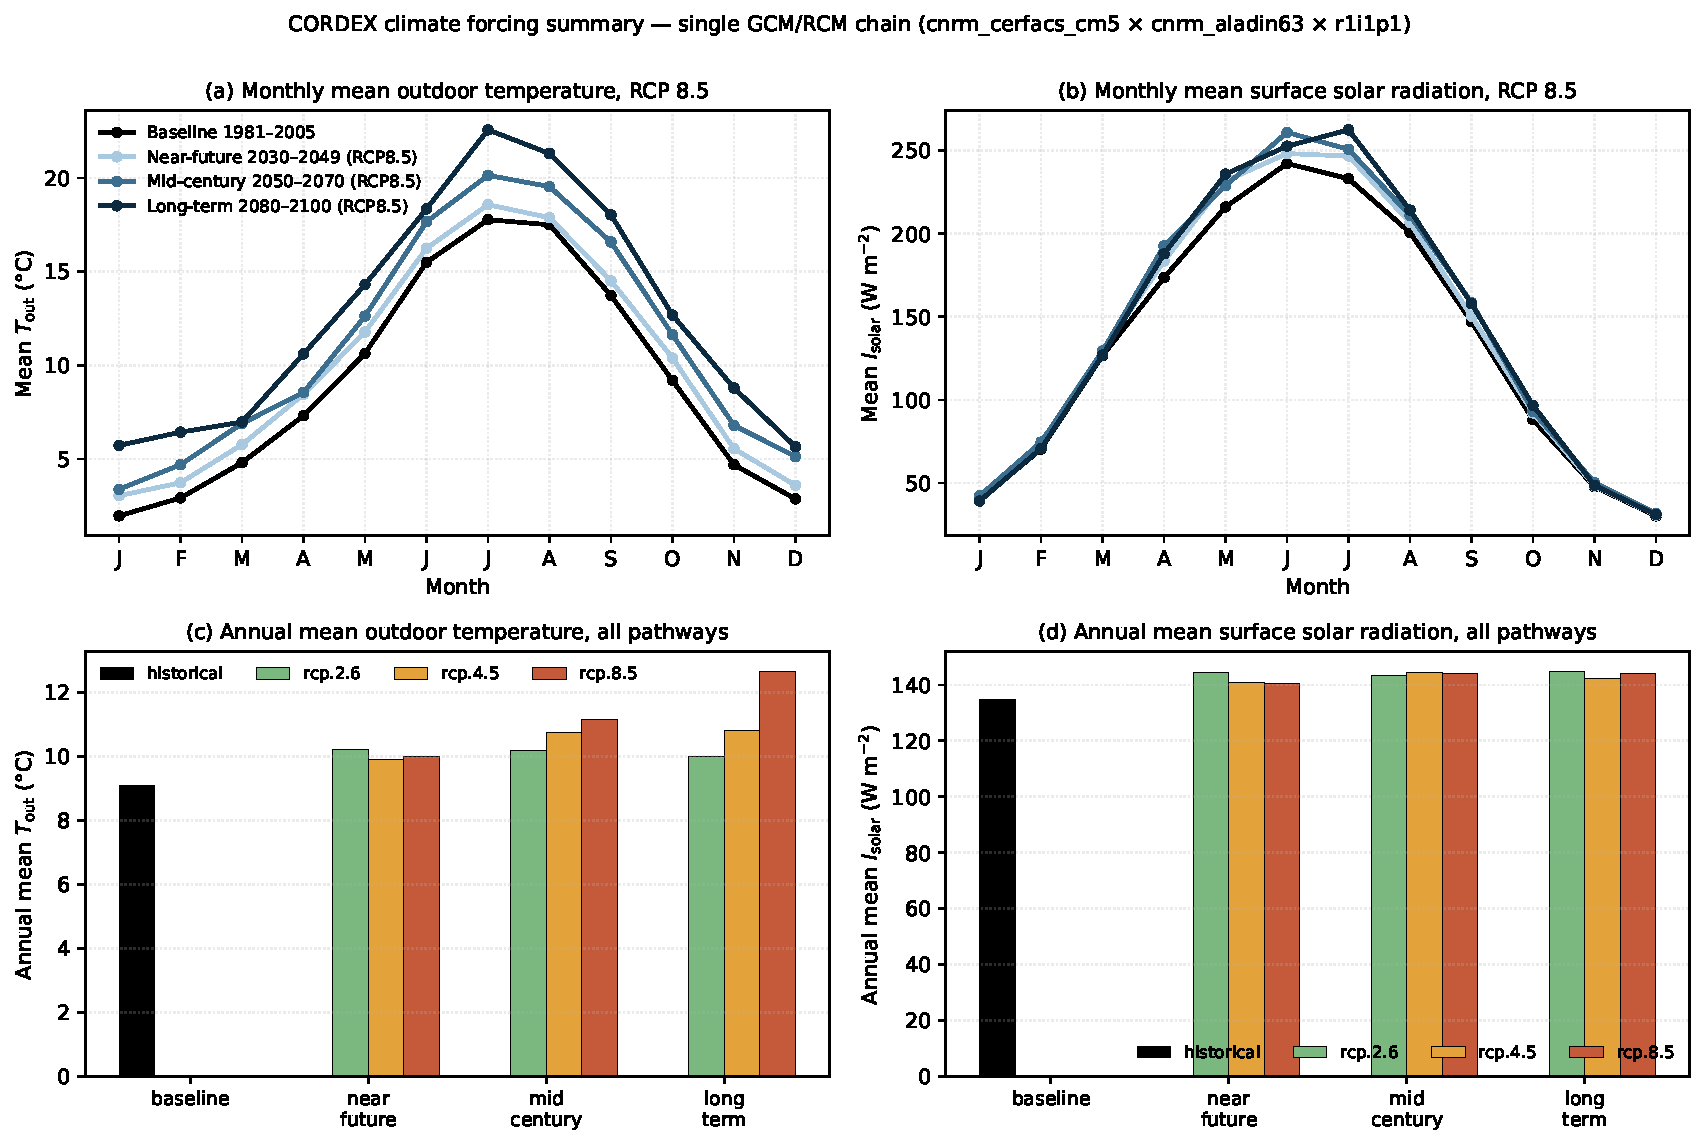
\includegraphics[width=\textwidth]{figures/climate_forcing_summary.pdf}
  \caption{CORDEX climate forcing summary, single GCM/RCM chain.}
  \label{fig:climate_forcing_summary}
\end{figure}

Panels (a) and (b) of \Cref{fig:climate_forcing_summary} show the monthly climatology of outdoor temperature and surface solar radiation for the baseline window (black) and the three future windows under RCP\,8.5 (blue shades, darker $=$ further future); the temperature signal concentrates in the warm half of the year.
\newline Panels (c) and (d) give annual means across the four windows and the historical, RCP\,2.6, RCP\,4.5, and RCP\,8.5 pathways: annual mean $T_{\text{out}}$ rises from $\sim\SI{9.1}{\celsius}$ at baseline to $\sim\SI{12.6}{\celsius}$ in the long-term RCP\,8.5 cell, while annual mean $I_{\text{solar}}$ stays within $\sim\SI{135}{\watt\per\square\meter}$ to $\sim\SI{145}{\watt\per\square\meter}$ across all futures.


\subsection{Macro \& Benchmark}
\label{sec:macro_benchmark}

Two configuration files anchor the model to Belgian macro evidence: the Eurostat \texttt{nrg\_d\_hhq} end-use shares for the Belgian and EU-27 residential sectors \cite{eurostat_disaggregated_nodate}, together with macro context from \texttt{ten00124}, \texttt{ten00123} and \texttt{ten00125} \cite{EurostatTen00124,EurostatTen00125}. The relevant Belgian shares are reproduced in \Cref{tab:macro_benchmark}.

\begin{table}[ht]
  \centering
  \footnotesize
  \caption{Belgian residential end-use shares and macro context.}
  \label{tab:macro_benchmark}
  \begin{tabular}{@{}l r l@{}}
    \toprule
    \textbf{Quantity} & \textbf{Value (\%)} & \textbf{Source} \\
    \midrule
    Space heating share        & 73.01 & \texttt{nrg\_d\_hhq} \\
    Water heating share        & 12.00 & \texttt{nrg\_d\_hhq} \\
    Cooking share              &  1.64 & \texttt{nrg\_d\_hhq} \\
    Space cooling share        &  0.07 & \texttt{nrg\_d\_hhq} \\
    Residual (appl.+light.+other) & 13.29 & \texttt{nrg\_d\_hhq} \\
    \midrule
    Residential share of final energy (BE, 2022)  & 24.0 & \texttt{ten00124} \\
    Electricity share of final energy (BE, 2022)  & 21.7 & \texttt{ten00123} \\
    Household electricity share (BE, 2022)        & 19.1 & \texttt{ten00125} \\
    \bottomrule
  \end{tabular}
\end{table}

\subsubsection*{Energy carriers \& technology}
The \texttt{belgian\_technology\_inputs.yaml} file records the Belgian carrier and technology metadata used by the technology cases of the \hyperref[sec:scenarioTreeSystem]{scenario tree}. It is compiled from the sources listed in \Cref{tab:belgian_tech_sources} and contains for each technology: a reference year, a low/base/high range and a suitability note. The headline carrier shares used as the canonical baseline are gas $0.637$, heating oil $0.211$, with the remainder split between electric, biomass, district heat and other, consistent with the \textcite{KBSFrb2024} and the JRC \cite{JRC2022HeatPumpBelgium}.

\begin{table}[ht]
  \centering
  \footnotesize
  \caption{Belgian technology evidence sources.}
  \label{tab:belgian_tech_sources}
  \begin{tabular}{@{}p{0.32\linewidth} p{0.20\linewidth} p{0.40\linewidth}@{}}
    \toprule
    \textbf{Source} & \textbf{Reference year} & \textbf{Used for} \\
    \midrule
    KBS-Frb Energy-Poverty Barometer \cite{KBSFrb2024}
      & $2022$ & main-heating carrier shares \\
    JRC Country Fiche: Belgian heat-pump market \cite{JRC2022HeatPumpBelgium}
      & $2022$ & gas-boiler / heat-pump installed stock \\
    RAP Country Report Belgium \cite{RAP2020BelgiumReport}
      & $2020$ & DHW carrier mix; district-heating context \\
    KU Leuven HP performance working paper \cite{KULeuvenHP2015}
      & $2015$ & Belgian heat-pump SPF ranges \\
    IEA PVPS Belgium 2024 \cite{IEAPVPS2024Belgium}
      & $2024$ & national cumulative PV capacity \\
    BRUGEL Annual Report \cite{Brugel2024Annual}
      & $2024$ & Brussels regional PV anchor \\
    Statbel EV stock \cite{Statbel2025EV}
      & $2025$ & BEV stock; registration split \\
    Statbel vehicles per household \cite{Statbel2024VehiclesHousehold}
      & $2024$ & car-ownership conditioning \\
    Federal carbon \& energy taxation landscape \cite{Climat2025Taxation}
      & $2025$ & EV annual distance; electricity intensity \\
    CRM Monitoring Report \cite{CRM2025Monitoring}
      & $2024$ & Flemish home-battery stock \\
    \bottomrule
  \end{tabular}
\end{table}

\subsubsection*{Energy shares}
The annual calibration baseline itself sits in \texttt{config/thesis.yaml}: annual electricity \SI{3500}{kWh} (\SIrange{3000}{3900}{kWh}), annual space heating \SI{12000}{kWh} (\SIrange{12000}{16000}{kWh}), and annual domestic hot water \SI{3000}{kWh} (\SIrange{2500}{3300}{kWh}). Electric DHW and space-heating shares are kept modest because thermal services are primarily represented through useful heat and carrier conversion rather than as dominant baseline electric loads. This decision is mainly driven by the fact that Belgian residential heating is gas-dominated: the main-heating carrier shares of $\sim$\SI{64}{\percent} gas and $\sim$\SI{21}{\percent} heating oil \cite{KBSFrb2024,JRC2022HeatPumpBelgium} leave only a small electric-heating minority, so the share of total electricity that goes to space heating in a representative dwelling is correspondingly small even though the share of total final energy going to space heating is large \cite{eurostat_disaggregated_nodate}.


\subsection{Smart Meter Data}
\label{sec:smartMeterData}

The smart-meter inputs serve various purposes and are kept
strictly separate.
 
\subsubsection*{Representative shape input} 
The Low Carbon London (LCL) dataset \cite{LowCarbonLondon2014} includes the load profiles of ${\sim}5500$ London households at \SI{30}{min} resolution, is stored as input-csv file, and is used inside the loader as a representative electrical load \emph{shape} that is subsequently rescaled to the Belgian annual baseline. LCL is deliberately treated as an internal shape source and is not used as thesis-facing aggregate validation evidence, because validating against the same family of data that supplies the input shape would not constitute an independent check.
 
\subsubsection*{Belgian aggregate validation} 
The Flemish DSO Fluvius publishes representative residential profiles disaggregated by heat-pump, EV and PV indicators \cite{Fluvius2024OpenData}. Eight combinations are stored under the fluvius-input file: \texttt{geen\_ZP}, \texttt{enkel\_ZP}, \texttt{WP\_geen\_ZP}, \texttt{WP\_met\_ZP}, \texttt{EV\_geen\_ZP}, \texttt{EV\_met\_ZP}, \texttt{WP\_EV\_geen\_ZP}, and \texttt{WP\_EV\_met\_ZP}\footnote{WP means ``warmtepomp''; meaning heat pump. ZP means ``zonnepanelen''; meaning PV panels.}. The schema is per connection-point (\texttt{EAN\_ID}\footnote{An EAN (European Article Number) is the unique 18-digit identifier of a physical electricity or gas connection point in the Belgian and Dutch markets, assigned by the distribution system operator (DSO). Each meter, and therefore each household, has one.}) \SI{15}{min} rows with consumption and injection plus equipment indicators. Fluvius profiles are the aggregate-validation source in \Cref{sec:validation}.
 
\subsubsection*{Belgian high-frequency case study} 
The KU\,Leuven three-house dataset \cite{KULeuven3House} provides high-frequency electrical (and partial gas) measurements for three Belgian dwellings, summarised in \Cref{tab:kul_houses}. The dataset is used only as a high-frequency event-realism check, validating ramps, spikes, daily peaks, etc. (\Cref{sec:validation}).

\begin{table}[ht]
  \centering
  \footnotesize
  \caption{KU\,Leuven three-house high-frequency dataset.}
  \label{tab:kul_houses}
  \begin{tabular}{@{}l l l l l@{}}
    \toprule
    \textbf{House} & \textbf{Type} & \textbf{EPC} &
      \textbf{Equipment} & \textbf{2023 coverage} \\
    \midrule
    1 & detached
      & A (\SI{39}{kWh/m^2})
      & PV, $\text{HP}_\text{geo}$, EV
      & six segments \\
    2 & apartment
      & B (\SI{162}{kWh/m^2})
      & none
      & three segments \\
    3 & attached
      & B (\SI{135}{kWh/m^2})
      & PV
      & one segment \\
    \bottomrule
  \end{tabular}
\end{table}

\subsubsection*{Belgian PV reference} 
The aggregate Belgian transmission-PV generation series published by Elia \cite{Elia2024PVODS032} is stored in the \texttt{ods032.csv} file at \SI{15}{min} resolution, with columns \texttt{measured}, \texttt{monitoredcapacity} and \texttt{loadfactor}. It is used as the country-level PV anchor for the PV triangle validation (\Cref{sec:validation}).


% Macro-level inputs are used as calibration anchors and plausibility context. The configuration contains annual baseline values for total household electricity, space heating, and domestic hot water, together with an electricity end-use split. During the annual simulation, Model v2 rescales modelled electricity end uses to the configured annual electricity targets. This means that the macro inputs constrain annual energy levels, while the hourly and sub-hourly temporal structure remains determined by the load-shape source, stochastic events, occupancy, thermal physics, and weather forcing.

% The repository also loads a Eurostat-derived household end-use table for Belgium and the EU-27 \cite{eurostat_disaggregated_nodate}. In the active data loader, the Belgian water-heating, cooking, and residual lighting/appliance shares are used to disaggregate the representative Low Carbon London aggregate electricity profile into appliances, lighting, cooking, and DHW components. The lighting share is further split from the combined appliance-lighting bucket using a configured fraction.

% For aggregate validation, the repository includes a Fluvius external validation path. The Fluvius loader reads quarter-hourly representative electricity profiles, converts interval energy to average power, groups profiles by technology category such as base, EV, heat pump, and combined EV/heat-pump, and constructs a weighted representative profile. The validation runner then scales both model and Fluvius profiles by the configured household count and compares absolute aggregate demand metrics. This is best interpreted as an aggregate-profile plausibility check rather than direct feeder validation, because the Fluvius inputs are representative profile data rather than a measured feeder serving the simulated households.

% \subsection{Smart-Meter Data}

% The model uses smart-meter data in two distinct ways. First, the active runtime load-shape source is the refactored Low Carbon London 2013 dataset. The loader reads the half-hourly household columns, computes the mean profile across meters, interprets the values as kWh per interval, converts them to average watts, and then splits the aggregate profile into end-use components using the Eurostat-derived shares. This profile is therefore an input shape source rather than an independent validation target. It should be noted that Low Carbon London should not be used as thesis-facing validation evidence in this configuration, because it already influences the modelled load shape \cite{tindemans2023lclRefactored}.

% Second, independent smart-meter or metered profile data are used for validation diagnostics. The KU Leuven validation path loads the PREMISES smart-meter measurements for three Belgian households \cite{palaciosGarcia2024premises}, detects whether each file contains direct power or cumulative energy, converts the signal to kW where needed, aggregates it to 15-minute mean power, maps the timestamps onto the model reference year, and compares the resulting profiles with model output. The validation metrics focus on high-frequency realism: daily maxima, spike counts, ramp rates, variance, skewness, kurtosis, and short visual segments. This dataset is therefore used as a case-study benchmark for event and ramp behaviour., not as a statistical calibration sample for the whole Belgian residential stock.

% The distinction between calibration and validation data is important. Low Carbon London contributes to the simulated temporal shape and is therefore part of the model input chain. Eurostat contributes annual and end-use calibration information. Fluvius and KU Leuven provide external plausibility checks at different aggregation levels: Fluvius for representative aggregate profiles and KU Leuven for high-frequency household event structure. This separation prevents the same data source from being treated simultaneously as an input and as independent evidence of model validity.


% \subsection{Preprocessing}
% %%% canonical timestamps
% %%% timezone handling
% %%% missing-data policy
% %%% reproducibility and audit trail



%%% --- %%%
\pagebreak
\section{Modelling Framework}
\label{sec:modelling_framework}

This subsection deconstructs the model architecture: how the inputs disclosed in \Cref{sec:model_inputs} are turned into per-timestep, per-household, per-scenario outputs. 
\newline The subsections below treat the layers in the order they execute (\hyperref[sec:archetypeConstruction]{archetype} $\to$ \hyperref[sec:occupancyStateModel]{occupancy} $\to$ \hyperref[sec:deterministicBaselineDemandModel]{deterministic baseline} $\to$ \hyperref[sec:stochasticScenarioGeneration]{stochastic cohort}), then describe the two outer wraps that vary the exogenous inputs (\hyperref[sec:climateScenariosFramework]{climate scenarios}, \hyperref[sec:climateUncertainty]{climate uncertainty}), and close with the output ledger.


\subsection{Archetype Construction}
\label{sec:archetypeConstruction}

The model represents the dwelling as one lumped thermal zone, fully described by a small parameter vector. \Cref{tab:archetype_params} lists the parameters that enter the physics layer. They are sourced from the \num{24}-row archetype table introduced in \Cref{sec:input_building_archetype} and from the companion envelope, internal-gain and airflow reference tables.

% \begin{table}[ht]
%   \centering
%   \footnotesize
%   \caption{Per-archetype parameter vector consumed by the physics
%   layer. Symbols match the variable names used in the implementation
%   (\texttt{src/model\_v3/interfaces.py}).}
%   \label{tab:archetype_params}
%   \begin{tabular}{@{}l l l@{}}
%     \toprule
%     \textbf{Symbol} & \textbf{Meaning} & \textbf{Source} \\
%     \midrule
%     $\text{stock\_weight}$
%       & weight in stock-weighted sampling
%       & Statbel dwelling stock \cite{Statbel2024Census} \\
%     $UA$ (\texttt{heat\_loss\_coefficient\_W\_per\_C})
%       & envelope conductance
%       & Belgian TABULA \cite{Cyx2011TABULABE} + reconstructed areas \\
%     $C$ (\texttt{thermal\_mass\_Wh\_per\_C}, \texttt{C\_J\_per\_K})
%       & effective thermal capacitance
%       & archetype default \\
%     $V$ (\texttt{volume\_m3})
%       & dwelling air volume
%       & reconstructed envelope geometry \\
%     $\text{ACH}_{\text{inf}}, \text{ACH}_{\text{vent,base/occ}}$
%       & infiltration and ventilation air-change rates
%       & Belgian airtightness anchors
%         ($\text{ACH}_{50}$ as-is $6.3$, renovated $2.5$)
%         \cite{Cyx2011TABULABE,Hens2007Airtightness}; ventilation
%         flow defaults from EN\,16798-1
%         \cite{EN16798_1_2019} \\
%     \texttt{ventilation\_type}, $\eta_{\text{HRV}}$
%       & ventilation regime, heat-recovery effectiveness
%       & EPB ventilation classes
%         \cite{VEKAEnergyPerformance,SPWEnergyPerformance};
%         $\eta_{\text{HRV}}$ from EN\,308 product range
%         \cite{EN308_HRV} \\
%     $Q_{\text{occ}}, Q_{\text{app}}, Q_{\text{light}}, Q_{\text{cook}}$
%       & internal gain references
%       & per-person sensible gains from ISO 13790 / EN\,16798-1
%         \cite{ISO13790_2008,EN16798_1_2019}; floor area from TABULA
%         type means \cite{Cyx2011TABULABE} \\
%     $T_{\text{set}}, T_{\text{min}}, T_{\text{max}}$
%       & comfort setpoint and band
%       & archetype comfort defaults \\
%     $Q_{\text{heat,max}}$, \texttt{heating\_cop}, \texttt{dhw\_cop}
%       & heating capacity and conversion COP
%       & technology case + heat-pump performance model \\
%     \bottomrule
%   \end{tabular}
% \end{table}

\begin{table}[ht]
  \centering
  \footnotesize
  \caption{Per-archetype parameter vector consumed by the physics
  layer. Symbols match the variable names used in the implementation.}
  \label{tab:archetype_params}
  \begin{tabular}{@{}p{0.27\linewidth} p{0.27\linewidth}
                   p{0.40\linewidth}@{}}
    \toprule
    \textbf{Symbol} & \textbf{Meaning} & \textbf{Source} \\
    \midrule
    $\text{stock\_weight}$
      & weight in stock-weighted sampling
      & Statbel dwelling stock \cite{Statbel2024Census} \\
    $UA$
      & envelope conductance
      & Belgian TABULA \cite{Cyx2011TABULABE} $+$ reconstructed areas \\
    $C$
      & effective thermal capacitance
      & archetype default \\
    $V$
      & dwelling air volume
      & reconstructed envelope geometry \\
    $\text{ACH}_{\text{inf}}, \text{ACH}_{\text{vent,base/occ}}$
      & infiltration and ventilation air-change rates
      & Belgian airtightness anchors
        ($\text{ACH}_{50}$ as-is $6.3$, renovated $2.5$)
        \cite{Cyx2011TABULABE,Hens2007Airtightness};
        ventilation defaults from EN\,16798-1
        \cite{EN16798_1_2019} \\
    \texttt{ventilation\_type}, $\eta_{\text{HRV}}$
      & ventilation regime, heat-recovery effectiveness
      & EPB classes
        \cite{VEKAEnergyPerformance,SPWEnergyPerformance};
        $\eta_{\text{HRV}}$ from EN\,308 \cite{EN308_HRV} \\
    $Q_{\text{occ}}, Q_{\text{app}}, Q_{\text{light}}, Q_{\text{cook}}$
      & internal gain references
      & per-person gains from ISO\,13790 / EN\,16798-1
        \cite{ISO13790_2008,EN16798_1_2019}; floor area from TABULA
        \cite{Cyx2011TABULABE} \\
    $T_{\text{set}}, T_{\text{min}}, T_{\text{max}}$
      & comfort setpoint and band
      & archetype comfort defaults \\
    \texttt{heating\_cop}, \texttt{dhw\_cop}
      & heating capacity and conversion COP
      & technology case $+$ heat-pump performance model \\
    \bottomrule
  \end{tabular}
\end{table}

\subsubsection*{Assignment modes}
Assignment from the building stock to one archetype follows three modes. The deterministic single-archetype mode builds one representative dwelling whose parameters are the stock-weighted average over the 24 rows. The deterministic single-row mode picks the most prevalent archetype. The stochastic mode draws one archetype per household with probability equal to its stock weight, so that the cohort population reproduces the Belgian dwelling-type and construction-period distribution in expectation.

\subsubsection*{Physical heterogeneity}
Independent physical heterogeneity is added on top of the archetype draw. The cohort sampler multiplies $UA$ by a normal scale factor ($\sigma_{UA}=0.25$), the thermal mass by a normal factor ($\sigma_{C}=0.20$), the infiltration rate by a log-normal factor ($\sigma_{\text{inf}}=0.40$), and the heating COP by a normal factor ($\sigma_{\text{COP}}=0.10$), each clipped to a physically meaningful range\footnote{Concrete bounds are encoded in the \texttt{sampler.py} file; e.g.\ the $UA$ scale is clipped to $[0.4, 2.0]$, infiltration to $[0.3, 3.5]$, COP to $[0.5, 1.5]$.}. This separation between archetype and per-household perturbation is what gives the cohort both Belgian-stock realism and within-stock variability.

\subsubsection*{Heating and emitter systems}
Each archetype is also paired with a heating-system class and an emitter type. Heating-technology probabilities can come from two sources: explicit \emph{technology-case} probabilities encoded by the scenario tree, and the Belgian carrier stock baseline from the Belgian technology inputs YAML file. The emitter family (underfloor, low-temperature radiator, standard radiator, high-temperature radiator, fan coil) is drawn from a configurable distribution and is the input to the weather-dependent heat-pump COP model (\Cref{sec:deterministicBaselineDemandModel}).


\subsection{Occupancy State Model}
\label{sec:occupancyStateModel}

Occupancy is modelled as a three-state homogeneous-in-day-type schedule, $\{\texttt{away},\texttt{awake},\texttt{sleep}\}$, at a \SI{15}{min} timestep, conditioned on weekday vs weekend. For each timestep, two sources combine to produce the state distribution. First, the configured time-of-day rules prescribe an absolute probability $p_{\text{rule}}(s)$ for some state $s$ (e.g.\ $P(\text{sleep} \mid 23\!:\!00\text{--}07\!:\!00, \text{weekday}) = 0.85$). Second, any remaining probability mass is allocated according to fallback weights for the day-type. The resulting three-state schedule follows the structure of multi-state occupancy models such as \textcite{Richardson2010_DomesticHighRes}, but transition persistence is represented indirectly through broad time-of-day windows and cohort-level schedule perturbations rather than through an explicit Markov stickiness matrix\footnote{The spec also records state-specific \texttt{stickiness} fields, intended as legacy Markov persistence parameters (higher for \texttt{sleep} than for \texttt{awake} on the plausible reasoning that sleep dwell times are longer than evening activity dwell times). They are not consumed by the active \texttt{forcing\_builder.py} loader and are therefore not used in the results of \Cref{ch:results}.}.

\subsubsection*{Household variability}
Household-specific variability is added at the cohort layer. Each household draws an occupancy-intensity scale, a $\pm\SI{2}{h}$ time-shift on the schedule, a state-duration log-normal scale, and a triple of log-normal state biases. The household's behavioural class (\texttt{low\_flat}, \texttt{workday\_absent}, \texttt{peak\_heavy\_family}, \texttt{daytime\_home}) further modulates the occupancy scaling factor, the appliance event intensity, and the peak sensitivity. Household size is drawn from a Belgian working distribution (1--7 persons) and is used to scale appliance and DHW activity through a sub-linear exponent (the \texttt{household\_size\_activity\_scale} factor is $(n_{\text{occ}}/n_{\text{ref}})^{0.65}$ with $n_{\text{ref}}=2$, clipped to $[0.55, 2.25]$); the choice of a sub-linear scaling reflects shared-load saturation effects observed in metered household samples \cite{Wilke2013StochasticOccupancy}. \Cref{tab:household_size_dist} shows the working Belgian distribution recorded in \texttt{config/thesis.yaml}. The rounded probabilities sum to $0.995$ and are renormalised at draw time. The values are anchored to Statbel household statistics for Belgium \cite{Statbel2024Households} and cross-checked against OECD family-composition data \cite{OECDFamilyDatabase}. Notably, the share of 1-person households dominates in Belgium. A residual cluster of 0.03 was used for 5+ persons per household (PPH).

\begin{table}[ht]
  \centering
  \footnotesize
  \caption{Household-size distribution used by the cohort sampler.}
  \label{tab:household_size_dist}
  \begin{tabular}{@{}c c@{}}
    \toprule
    \textbf{PPH} & \textbf{Probability}\\
    \midrule
    1 & 0.360 \\
    2 & 0.310 \\
    3 & 0.145 \\
    4 & 0.110 \\
    5 & 0.040 \\
    6 & 0.020 \\
    7 & 0.010 \\
    \bottomrule
  \end{tabular}
\end{table}

The occupancy state is the coupling point between behaviour and physics. It drives the active ventilation regime, the internal-gain magnitudes, the appliance and DHW event-generation rates, and the active setpoint via the schedule state (\texttt{occupied\_day}, \texttt{evening}, \texttt{sleep}).

\subsubsection*{Occupancy state coupling}
\Cref{fig:occupancy_coupling} sketches how the sampled occupancy state is consumed by four downstream layers in each timestep: ventilation regime, internal gains, appliance/DHW event rates, and active thermostat setpoint. This coupling allows behaviour to affect both electrical end-use timing and thermal demand without merging the behaviour, physics, and control code paths.

\begin{figure}[ht]
  \centering
  \begin{tikzpicture}[
      every node/.style={font=\scriptsize, align=center, inner sep=3pt},
      hub/.style={draw, rounded corners=3pt, fill=black!4,
                  minimum width=6.0cm, minimum height=10mm,
                  font=\footnotesize\bfseries},
      input/.style={draw, rounded corners=2pt,
                    minimum width=6.0cm, minimum height=7mm,
                    font=\scriptsize\itshape},
      outblock/.style={draw, rounded corners=2pt,
                       minimum width=3.4cm, minimum height=15mm},
      arrow/.style={-{Latex[length=1.6mm]}, semithick, draw=black!75},
      node distance=4mm and 4mm,
  ]
    \node[input] (rules)
      {(hour, day type) $\to$ time-of-day rule + fallback};
    \node[hub, below=of rules] (state)
      {Occupancy state at $t$:
       $\bigl(P_{\text{away}},P_{\text{awake}},P_{\text{sleep}}\bigr)$,
       \texttt{schedule\_state}};
    \draw[arrow] (rules) -- (state);
 
    \node[outblock, below=10mm of state, xshift=-5.7cm] (set)
      {Active setpoint\\$T_{\text{set}}(t)$\\[1pt]
       \emph{ex: \texttt{evening}}\\\emph{$\Rightarrow$ \SI{21}{\celsius}}};
    \node[outblock, below=10mm of state, xshift=-1.9cm] (vent)
      {Ventilation regime\\$\text{ACH}_{\text{vent}}$\\[1pt]
       \emph{ex: occupied}\\\emph{$\Rightarrow$ $\text{ACH}_{\text{vent,occ}}$}};
    \node[outblock, below=10mm of state, xshift= 1.9cm] (gain)
      {Internal gain\\$Q_{\text{int}}(t)$\\[1pt]
       \emph{ex: 4 occupants}\\\emph{$\approx\SI{292}{\watt}$}};
    \node[outblock, below=10mm of state, xshift= 5.7cm] (evt)
      {Event intensity\\$\lambda(t)$\\[1pt]
       \emph{ex: $P_{\text{awake}}\!\cdot\!m_{\text{class}}$}\\
       \emph{$\approx 1.28$}};
 
    \draw[arrow] (state) -- (set);
    \draw[arrow] (state) -- (vent);
    \draw[arrow] (state) -- (gain);
    \draw[arrow] (state) -- (evt);
  \end{tikzpicture}
  \caption{Occupancy state as the coupling point between behaviour
  and physics.}
  \label{fig:occupancy_coupling}
\end{figure}



\subsection{Deterministic Baseline Demand Model}
\label{sec:deterministicBaselineDemandModel}

The deterministic baseline is one dwelling running through the configured year hour by hour, with the indoor temperature and thermostat state carried forward across timesteps. It is implemented by \texttt{simulation/annual\_runner.py} as a sequence of four layers per timestep.

\subsubsection*{Physics layer}
The lumped-zone thermal balance integrates indoor temperature $T_{\text{in}}$ over the timestep $\Delta t$ with an adaptive explicit substep:
\begin{equation}
  C\,\frac{\mathrm{d}T_{\text{in}}}{\mathrm{d}t}
  = \underbrace{(UA + H_{\text{ve}})\,(T_{\text{out}} - T_{\text{in}})}_{\text{losses}}
  + \underbrace{Q_{\text{int}} + Q_{\text{sol}}}_{\text{gains}}
  + Q_{\text{heat}},
  \label{eq:thermal_balance}
\end{equation} where $H_{\text{ve}} = \rho\, c_p\, \dot V_{\text{eff}}$ is the ventilation-and-infiltration heat-transfer coefficient, $\dot V_{\text{eff}} = \dot V_{\text{inf}} + (1 - \eta_{\text{HRV}})\, \dot V_{\text{vent}}$ for a balanced system with heat recovery (and $\dot V_{\text{inf}} + \dot V_{\text{vent}}$ otherwise), $Q_{\text{int}}$ aggregates occupant, appliance, lighting and cooking gains, and $Q_{\text{sol}}$ is the orientation-resolved solar gain. The integration is performed with a stability-bounded explicit Euler scheme: the runner computes a stability factor $(UA + H_{\text{ve}})\,\Delta t / C$ and subdivides the timestep into substeps until the per-substep factor is below \num{0.5}, so the integrator is numerically stable even for low-mass or highly conductive archetypes.
\newline The free-float indoor temperature, i.e., the temperature the zone reaches in the timestep with $Q_{\text{heat}}=0$, is computed first. The heating demand is then the deficit between setpoint and free-float:
\begin{equation}
  Q_{\text{heat,demand}}
  = \max\!\left(0,\; \frac{C\,(T_{\text{set}} - T_{\text{free}})}{\Delta t}\right)
  \label{eq:heating_demand}
\end{equation}

\subsubsection*{Control layer}
The thermostat applies symmetric hysteresis around the active setpoint, with a configurable deadband (default $\delta = \pm \SI{0.75}{\celsius}$). The heating-on state is sticky: a household sampled with deadband $\delta$ switches the heater on when $T_{\text{in}} < T_{\text{set}} - \delta$ and off when $T_{\text{in}} > T_{\text{set}} + \delta$. The active setpoint itself is time-of-day-dependent: a per-household schedule sampled from:
\begin{align*}
    T_{\text{night}} \sim \mathcal{U}(16,18)\,\si{\celsius}\\
    T_{\text{day}} \sim \mathcal{U}(18,20)\,\si{\celsius}\\
    T_{\text{evening}} \sim \mathcal{U}(20,22)\,\si{\celsius},
\end{align*}
with class-conditional narrowing for \texttt{workday\_absent} and \texttt{daytime\_home} households, and daily overrides drawn with $P=0.10$--$0.20$ for $\pm\SI{1}{\celsius}$--$\SI{2}{\celsius}$ shifts over a $3$--$7$-hour window.
\newline An optional cooling-oriented window-opening event boosts the air-change rate when the zone is occupied, in the \texttt{occupied\_day} state, with $T_{\text{in}} > T_{\text{set,high}} + \theta_{\text{trig}}$ and a positive indoor--outdoor gradient. The extra ACH is configurable (default $+0.5$).

\subsubsection*{Systems layer}
The heating dispatcher splits the requested useful heat across carriers under the active technology case. For non-electrified carriers (gas, oil, biomass, propane, coal, district heat) it applies the carrier-specific conversion efficiency. For heat pumps, the model computes one effective COP per timestep from the implemented performance curve in \texttt{heat\_pump\_performance.py}.

\paragraph{Hydronic heat pumps.}
For hydronic heat pumps, the sink temperature follows an emitter weather curve:
\begin{equation}
\begin{aligned}
  f_T(t)
  &= \mathrm{clip}\!\left(
      \frac{T_{\mathrm{mild}} - T_{\mathrm{out}}(t)}
           {T_{\mathrm{mild}} - T_{\mathrm{design}}},
      0, 1
    \right),\\
  T_{\mathrm{sink}}(t)
  &= T_{\mathrm{sink,low}}
    + f_T(t)\bigl(T_{\mathrm{sink,high}} - T_{\mathrm{sink,low}}\bigr),
\end{aligned}
  \label{eq:hp_sink_weather_curve}
\end{equation}
with default $T_{\mathrm{design}}=-\SI{7}{\celsius}$ and $T_{\mathrm{mild}}=\SI{15}{\celsius}$. Air-to-air heat pumps use the indoor setpoint as sink temperature, and heat-pump water heaters use the configured tank/sink temperature.
The base COP is a clipped\footnote{Here, clipping means bounding a computed value to an allowed interval: values below the lower bound are set to the lower bound, and values above the upper bound are set to the upper bound. It prevents physically implausible COP values while leaving the linear correction unchanged inside the calibrated range.} linear correction around the technology reference point:
\begin{equation}
\begin{aligned}
  \mathrm{COP}_{\mathrm{base}}(t)
  &= \mathrm{clip}\!\left[
      \mathrm{COP}_{\mathrm{ref}}
      + a_{\mathrm{src}}\bigl(T_{\mathrm{src}}(t)-T_{\mathrm{src,ref}}\bigr)
      \right.\\
  &\qquad \left.
      - a_{\mathrm{sink}}\bigl(T_{\mathrm{sink}}(t)-T_{\mathrm{sink,ref}}\bigr),
      \mathrm{COP}_{\min}, \mathrm{COP}_{\max}
    \right].
\end{aligned}
  \label{eq:hp_cop_base}
\end{equation}

\paragraph{Air-source heat pumps.}
For air-source heat pumps $T_{\mathrm{src}}(t)=T_{\mathrm{out}}(t)$; for \texttt{ground\_source} it is the configured ground-source temperature; and for heat-pump water heaters it is the configured ambient source temperature.
\newline Two multiplicative factors are then applied. The defrost factor is
\begin{equation}
  F_{\mathrm{def}}(t)
  =
  \begin{cases}
    1-d, & \text{air-source heating and } -\SI{3}{\celsius}
      \le T_{\mathrm{src}}(t) \le \SI{6}{\celsius},\\
    1, & \text{otherwise},
  \end{cases}
  \label{eq:hp_defrost}
\end{equation}
and the part-load factor is derived from
\begin{equation}
\begin{aligned}
  \mathrm{PLR}(t)
  &= \mathrm{clip}\!\left(\frac{Q_{\mathrm{useful}}(t)}
                                {Q_{\mathrm{cap}}(t)},0,1\right),\\
  g_{\mathrm{PL}}(t)
  &= 1-(1-\eta_{\mathrm{PL}})
      \left(1-\frac{\mathrm{PLR}(t)}{\mathrm{PLR}_{\min}}\right),\\
  F_{\mathrm{PL}}(t)
  &=
  \begin{cases}
    1, & \mathrm{PLR}(t) \ge \mathrm{PLR}_{\min},\\
    \mathrm{clip}\!\left(g_{\mathrm{PL}}(t),\eta_{\mathrm{PL}},1\right),
      & \mathrm{PLR}(t) < \mathrm{PLR}_{\min}.
  \end{cases}
\end{aligned}
  \label{eq:hp_part_load}
\end{equation}
The effective COP and electrical heat-pump demand are therefore:
\begin{equation}
\begin{aligned}
  \mathrm{COP}_{\mathrm{eff}}(t)
  &= \mathrm{clip}\!\left[
      \mathrm{COP}_{\mathrm{base}}(t)
      F_{\mathrm{def}}(t)F_{\mathrm{PL}}(t),
      \mathrm{COP}_{\min}, \mathrm{COP}_{\max}
    \right],\\
  P_{\mathrm{el,HP}}(t)
  &= \frac{Q_{\mathrm{useful,HP}}(t)}
         {\mathrm{COP}_{\mathrm{eff}}(t)}.
\end{aligned}
  \label{eq:hp_effective_cop}
\end{equation}
The low-temperature capacity fraction is recorded separately as an availability diagnostic used by dispatch, not as an extra COP multiplier. Default COP envelopes follow literature ranges for residential air-to-water, air-to-air, ground-source and heat-pump water heaters \cite{KULeuvenHP2015,Stafford2017HPField}. The active heat-pump spec, refrigerant, emitter, source/sink temperatures, and COP terms are written to the system-state metadata.

\paragraph{Ground-source heat pump}
The \texttt{ground\_source} configuration is treated as a generic ground-source-to-water heat pump with a $B0/W35$ reference point in line with EN\,14511 \cite{EN14511_2018}: source reference \SI{0}{\celsius}, sink reference \SI{35}{\celsius}, $\mathrm{COP}_{\mathrm{ref}}=3.8$, and R\,290 refrigerant. R\,290 is used as a representative low-GWP refrigerant for the future heat-pump stock rather than as a simulated cycle variable.\footnote{The model records the refrigerant label in the heat-pump metadata, but it does not simulate refrigerant charge, leakage, safety constraints, or vapour-compression cycle physics. The R\,290 choice therefore prevents the future heat-pump cases from implicitly relying on high-GWP legacy refrigerants without expanding the model boundary to component-level HVAC design.} The source loop is abstracted to a configured ground temperature (default \SI{8}{\celsius}); vertical-borehole, horizontal-collector, and open-loop designs are not distinguished because they require soil, borehole, and aquifer inputs outside the residential demand boundary. This abstraction is consistent with using ground-source heat pumps as a representative technology class rather than as component-level HVAC design \cite{JRC2022HeatPumpBelgium}.

\subsubsection*{Final annual electricity}
Final-energy electricity is aggregated as:
\begin{equation}
  P_{\text{el,gross}} = P_{\text{el,SH}} + P_{\text{el,DHW}}
  + P_{\text{el,app}} + P_{\text{el,light}}
  + P_{\text{el,cook}} + P_{\text{el,EV}},
\end{equation}
PV self-consumption is subtracted at the dwelling meter:
\begin{equation}
  P_{\text{el,grid,import}}
    = \max\!\bigl(0,\; P_{\text{el,gross}} - P_{\text{pv}}\bigr),
  \qquad
  P_{\text{el,grid,export}}
    = \max\!\bigl(0,\; P_{\text{pv}} - P_{\text{el,gross}}\bigr),
\end{equation}
and parallel carrier-specific power columns ($P_{\text{gas,SH}}, P_{\text{gas,DHW}}, P_{\text{oil,SH}}, P_{\text{oil,DHW}}, \ldots, P_{\text{district,DHW}}$) are kept first-class for the scenario-tree comparisons.

\subsubsection*{End-use rescaling}
The annual electricity total is rescaled to the configured Belgian baseline; the rescaling factor is recorded per household and per cohort so that calibrated and pre-calibration diagnostics can be separated in \Cref{sec:validation}. Heating thermal demand is similarly anchored to the Eurostat-derived BE end-use share (\Cref{tab:macro_benchmark}) through the envelope calibration factor.



\subsection{Stochastic Scenario Generation}
\label{sec:stochasticScenarioGeneration}

The cohort layer wraps the deterministic baseline. Given a reproducible seed, it samples $N$ independent household parameter vectors, runs each through the annual runner, and aggregates the cohort by summation. The independent draws cover four blocks: a physical block (archetype, $UA$ scale, thermal-mass scale, infiltration, COP scale), a behavioural block (occupancy intensity, schedule shift, household class, household size, DHW intensity and event rate, appliance intensity, dryer presence), a technology block (heating-technology probabilities under the active technology case, emitter type, refrigerant, heating-capacity scale, PV and EV ownership flags), and a control block (deadband, time-of-day setpoint schedule, daily overrides).

\subsubsection*{Behavioural uncertainty}
Behavioural uncertainty enters through occupancy-conditioned event generation rather than through independent average profiles. Appliance and DHW events are sampled on an internal sub-timestep grid, aggregated back to the active output timestep, and scaled by household class, occupancy state, end-use intensity parameters, and a sampled household random effect $u \sim \mathcal{N}(0,\sigma_h^2)$. Event starts are implemented as discrete Bernoulli trials with per-bin probability derived from the local event rate, not as a continuous-time Poisson process; the generated profiles are then reconciled with the model's configured annual end-use calibration where that calibration path is active.
\newline \Cref{fig:event_generator_intensity} visualises the expected appliance-event intensity used by this layer. The diagnostic intensity follows the hour-resolved \texttt{awake}-state probability from \Cref{sec:occupancyStateModel} and the class multipliers $m_{\text{low\_flat}}=0.7$, $m_{\text{workday\_absent}}=0.95$, $m_{\text{daytime\_home}}=1.2$, and $m_{\text{peak\_heavy\_family}}=1.5$. It should therefore be read as an expected-rate diagnostic, not as a realised event trace.

\begin{figure}[ht]
  \centering
  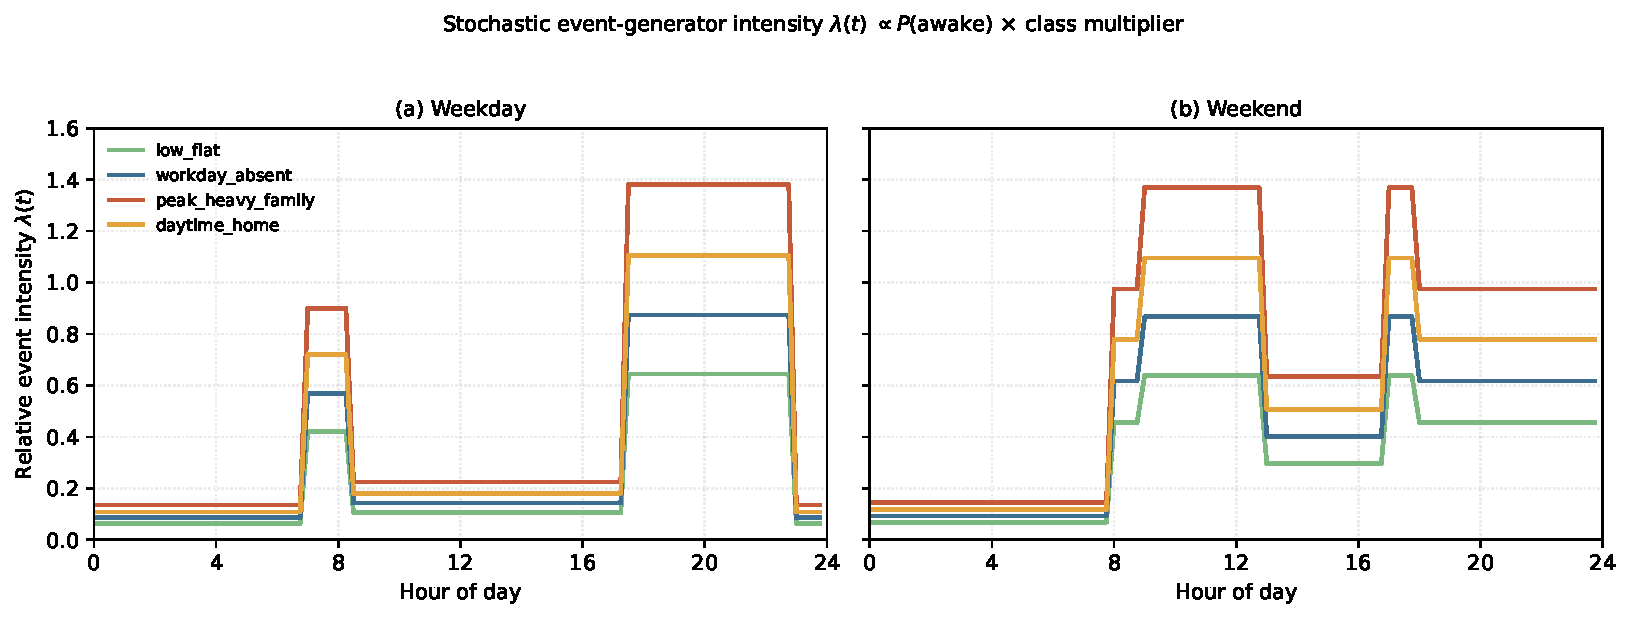
\includegraphics[width=\textwidth]{figures/event_generator_intensity.pdf}
  \caption{Expected event-generator intensity $\lambda(t) \propto P(\text{awake}\mid t) \times m_{\text{class}}$ by hour of day, derived from the occupancy schedule rules in \texttt{occupancy\_model\_spec.yaml} and the four behavioural-class multipliers in \texttt{household\_classifier.py}.}
  \label{fig:event_generator_intensity}
\end{figure}



\subsubsection*{Cohort pipeline}
The canonical cohort is $N=30$ households, which is small enough to keep single-configuration runs and validation workflows tractable. Stochastic spread within a scenario is captured by the realisation pool, which is enumerated as $100$ reproducible seeds (\texttt{seed\_0000}--\texttt{seed\_0099}); each seed generates an independent $N=30$ cohort, so a scenario with $k$ executed seeds aggregates $k \times 30$ household-years of stochastic samples. \Cref{fig:cohort_pipeline} sketches the cohort pipeline.

\begin{figure}[ht]
  \centering
  \resizebox{0.95\textwidth}{!}{%
  \begin{tikzpicture}[
      every node/.style={font=\scriptsize, align=center, inner sep=3pt},
      box/.style={draw, rounded corners=2pt,
                  minimum height=6.5mm, minimum width=2.6cm},
      stack/.style={box, fill=black!4},
      arrow/.style={-{Latex[length=1.4mm]}, semithick, draw=black!75},
      brace/.style={decorate, decoration={brace, amplitude=4pt}},
  ]
    \node[box] (seed) {Realization\\seed $s$};
    \node[box, right=8mm of seed] (samp) {Per-household\\sampler};
    \node[stack, right=10mm of samp] (hh1) {Household 1};
    \node[stack, below=1.5mm of hh1] (hh2) {Household 2};
    \node[font=\scriptsize, below=0mm of hh2] (dots) {$\vdots$};
    \node[stack, below=4mm of hh2] (hhN) {Household $N$};
    \node[box, right=12mm of hh1, yshift=-9mm] (run) {Annual runner};
    \node[box, right=8mm of run] (agg) {Cohort\\aggregate};
 
    \draw[arrow] (seed) -- (samp);
    \draw[arrow] (samp.east) -- (hh1.west);
    \draw[arrow] (samp.east) -- (hh2.west);
    \draw[arrow] (samp.east) -- (hhN.west);
    \draw[arrow] (hh1.east) -- (run.west);
    \draw[arrow] (hh2.east) -- (run.west);
    \draw[arrow] (hhN.east) -- (run.west);
    \draw[arrow] (run) -- (agg);
 
    \node[font=\scriptsize\itshape, below=2mm of run]
      {};
  \end{tikzpicture}}
  \caption{Stochastic cohort pipeline.}
  \label{fig:cohort_pipeline}
\end{figure}


\subsection{Climate Scenarios}
\label{sec:climateScenariosFramework}

Climate forcing for the scenario-tree leaves is derived from EURO-CORDEX \cite{Jacob2014EuroCordex} regional projections of 2-metre air temperature (\texttt{tas}) and surface solar radiation downwards (\texttt{rsds}). The forcing files described in \Cref{tab:climate_inventory} feed the annual runner through the same forcing-builder layer as the historical Uccle weather, so that the physics, control and systems code paths are identical for historical and future runs.

\subsubsection*{Window definitions} 
The four canonical analysis windows are a baseline ($1981$--$2005$), a near-future window ($2030$--$2049$), a mid-century window ($2050$--$2070$), and a long-term window ($2080$--$2100$), all with inclusive start and inclusive end. The baseline window is bounded above at $2005$ because the EURO-CORDEX historical experiment ends in $2005$, while RCP scenario simulations start in $2006$; aligning the baseline with the historical experiment avoids mixing historical and scenario forcing in the reference climate, while preserving a multi-decadal record that is long enough to characterise baseline thermal forcing. 

\subsubsection*{Pathways and technology pairing} 
Future windows are combined with three RCP pathways (\texttt{rcp\_2\_6}, \texttt{rcp\_4\_5}, \texttt{rcp\_8\_5}), in line with the canonical low/medium/high forcing trilogy \cite{vanVuuren2011}; the baseline window is restricted to the \texttt{historical} pathway. While newer scenario frameworks combine RCPs with Shared Socio-economic Pathways (SSP--RCP, \cite{Riahi2017SSP}), the present work isolates the effect of climate forcing on residential demand, with technology and behaviour treated as separate explicit dimensions of the scenario tree; RCP-only forcing is adequate for the restricted aim of isolating physical climate forcing, provided socio-economic interpretation is limited.

\subsubsection*{Scenarios}
The baseline scenario \texttt{baseline\_1981\_2005\_\_historical\_\_tech\_current\_stock} is a historical-climate reference case: the current Belgian stock representation is exposed to the $1981$--$2005$ historical climate window. It functions as a counterfactual reference for isolating climate and technology effects in \Cref{ch:results}; it is not a reconstruction of actual Belgian residential demand in $1981$--$2005$, because the technology stock of the early $1980$s differs from the current stock represented by \texttt{tech\_current\_stock}. In future windows, \texttt{tech\_frozen\_stock} is used as an explicit climate-only control: it holds the present-day technology representation fixed so that climate effects can be separated from electrification effects. It is not interpreted as a realistic future stock forecast.


\subsection{Climate Uncertainty}
\label{sec:climateUncertainty}

The scenario tree resolves three of the four classical sources of climate-impact uncertainty \cite{Hawkins2009UncertaintyPartitioning}: scenario uncertainty through the RCP pathways, technology/socio-economic uncertainty through the technology cases, and behavioural/internal variability through the stochastic seeds. The fourth source, climate-model structural uncertainty, is \emph{not} resolved: the current scenario tree uses one GCM/RCM chain, as mentioned in \Cref{sec:weatherClimate}. The results of \Cref{ch:results} are therefore conditional on this chain and should be read as such. This is a deliberate scoping choice. The CORDEX archive supports a multi-model ensemble for the same EUR-11 domain \cite{Jacob2014EuroCordex}, and the \texttt{src/climate/} pipeline is parametrised over the GCM/RCM identifiers, so adding more chains is a configuration extension rather than a code change. With $2800$ leaves already enumerated for one chain, adding $k$ additional chains multiplies the experiment space by $k$; the present work treats single-chain experiments as a defensible conditional estimate of demand response and flags multi-chain spread as the primary structural extension for \hyperref[sec:futurework]{future work}.

Two further interpretive notes follow from this scoping. First, the RCP pathways are read as conditional scenarios, not as probabilistic forecasts, consistent with the IPCC framing \cite{IPCC2014SynthesisReport}; no probability weights are attached to RCP\,2.6, RCP\,4.5, RCP\,8.5 in any of the comparisons. Second, the daily temporal resolution of the CORDEX product propagates a known smoothing: sub-daily peak demand is therefore reported only for the historical Uccle path and is not extrapolated to future windows, while daily and seasonal statistics are reported for all windows. \Cref{fig:climateUncertainty_scope} summarises which uncertainty sources are resolved by the scenario tree, and which are not.

\begin{figure}[ht]
  \centering
  \resizebox{0.98\textwidth}{!}{%
  \begin{tikzpicture}[
      every node/.style={font=\scriptsize, align=center, inner sep=3pt},
      box/.style={draw, rounded corners=2pt,
                  minimum height=8mm, minimum width=3.0cm},
      yes/.style={box, fill=black!5},
      no/.style={box, dashed, draw=black!50, text=black!60, font=\scriptsize\itshape},
      arrow/.style={-{Latex[length=1.4mm]}, semithick, draw=black!75},
  ]
    \node[yes] (scen) {Scenario\\uncertainty\\(RCP pathways)};
    \node[yes, right=8mm of scen] (tech) {Technology /\\socio-economic\\(technology cases)};
    \node[yes, right=8mm of tech] (beh)  {Behavioural /\\internal variability\\(stochastic seeds)};
    \node[no,  right=8mm of beh]  (mod)  {Climate-model\\structural\\(GCM/RCM ensemble)};

    \node[font=\scriptsize\itshape, above=1mm of scen] {resolved};
    \node[font=\scriptsize\itshape, above=1mm of tech] {resolved};
    \node[font=\scriptsize\itshape, above=1mm of beh]  {resolved};
    \node[font=\scriptsize\itshape, above=1mm of mod, text=black!70]
      {not resolved};
  \end{tikzpicture}}
  \caption{Sources of climate-impact uncertainty resolved by the scenario tree. The three resolved sources are the RCP pathways, the technology cases, and the stochastic seeds; the unresolved source is climate-model structural uncertainty, which is held fixed at one GCM/RCM chain in the present work.}
  \label{fig:climateUncertainty_scope}
\end{figure}


\subsection{Model Outputs}
\label{sec:modelOutputs}
A single ledger of outputs is produced regardless of which workflow generated the run; the workflow only changes which subset is treated as canonical and, for the scenario tree, which enumerated leaves were actually executed.
\Cref{tab:outputs_inventory} groups the output columns by family. Each column is exposed at the active simulation timestep: hourly for the historical-weather configuration and daily for the processed CORDEX scenario-tree leaves unless an explicit timestep override is configured.

\begin{table}[ht]
  \centering
  \footnotesize
  \caption{Output ledger produced by the systems layer.}
  \label{tab:outputs_inventory}
  \begin{tabular}{@{}l p{0.55\linewidth}@{}}
    \toprule
    \textbf{Family} & \textbf{Columns} \\
    \midrule
    Thermal state and comfort
      & $T_{\text{in,next}}$,
        $Q_{\text{heat,requested}}, Q_{\text{heat,supplied}},
        Q_{\text{heat,max}}, Q_{\text{unmet}}, Q_{\text{excess}}$,
        comfort violation $^{\circ}\text{C}$ and degree-hours \\
    Electricity by end use
      & $P_{\text{el,SH}}, P_{\text{el,DHW}}, P_{\text{el,app}},
         P_{\text{el,light}}, P_{\text{el,cook}}, P_{\text{el,EV}},
         P_{\text{el,total}}$ \\
    Distributed energy
      & $P_{\text{pv}}, P_{\text{el,gross}},
         P_{\text{el,net,grid}}, P_{\text{el,grid,import}},
         P_{\text{el,grid,export}}$ \\
    Non-electric carriers (SH and DHW)
      & $P_{\text{gas}}, P_{\text{oil}}, P_{\text{biomass}},
         P_{\text{propane}}, P_{\text{coal}},
         P_{\text{district\_heat}}$ \\
    Heat-pump diagnostics
      & effective COP, emitter, refrigerant, source/sink
        temperatures, defrost factor, part-load factor,
        capacity-available fraction \\
    Provenance
      & run id, artifact labels, run mode,
        \texttt{scenario\_leaf\_id}, technology case, seed,
        cohort size, config and input hashes
        \cite{Wilkinson2016} \\
    \bottomrule
  \end{tabular}
\end{table}

Three canonical aggregations of this ledger are produced. 
\newline The \emph{deterministic} aggregation is the annual single-household run under one weather year; it is used to inspect end-use shares, seasonal load shape, and comfort under one explicit configuration. 
\newline The \emph{stochastic} aggregation is the per-cohort statistics over the $N$-household sample for one configuration; it is used to characterise diversity, peak coincidence, and the spread of cohort totals. 
\newline The \emph{scenario-tree} aggregation is the same aggregation procedure applied to executed leaves of the four-dimensional tree and joined into a single comparison ledger by the standardised summary layer. The full scenario-tree design enumerates $2800$ possible leaves (\Cref{sec:scenarioTreeSystem}), but the thesis run set executes a targeted subset of $180$ leaves: $100$ full-window climate-only leaves and $80$ hourly design-year leaves. Results in \Cref{ch:results} therefore refer to this executed subset, not to a complete traversal of the full scenario tree.

Each run also writes a \texttt{run\_manifest.json} alongside the data outputs, recording the run mode, timestamp, configuration path and name, reference year, cohort size, random seeds, climate settings, key configured input paths, the resulting output artefact paths, and the git commit hash when the workspace exposes one. The manifest is the operational anchor of the reproducibility contract introduced in \Cref{sec:scenarioTreeSystem}: any output cell can be traced back to its config, inputs, and code state through the manifest alone.

% Climate forcing is derived from EURO-CORDEX simulations driven by Representative Concentration Pathways (RCPs). While newer scenario frameworks combine RCPs with Shared Socioeconomic Pathways (SSPs), the present work focuses on isolating the impact of climate variability on residential energy demand. As such, RCP-based climate projections are sufficient, since socio-economic factors such as building stock evolution and behavioural change are not explicitly modelled. The use of CORDEX ensures that these climate projections are available at a spatial and temporal resolution suitable for building-scale simulation.
% While SSP–RCP combinations are increasingly used in integrated assessment studies, the present work isolates the effect of climate forcing on residential demand. Therefore, RCP-based CORDEX simulations are used without explicit coupling to socio-economic pathways.
% the current scenario tree varies: climate window, RCP pathway, technology case, an stochastic seed
% but it does not yet vary the climate-model chain. So it represents RCP/window uncertainty conditional on one GCM-RCM chain, not the full spread across multiple climate models. A stronger climate uncertainty analysis would add more GCM/RCM chains.

% The baseline is a historical-climate reference case: the current-stock residential technology representation is exposed to the 1981-2005 historical climate window. It is used as a counterfactual reference for isolating climate and technology effects, not as a reconstruction of actual Belgian residential demand in 1981-2005.

% The baseline climate period was defined as 1981–2005 because it lies entirely within the EURO-CORDEX historical experiment, whereas RCP scenario simulations start in 2006. This avoids mixing historical and scenario-forced simulations in the reference climate, while still providing a sufficiently long multi-decadal period for estimating baseline thermal forcing conditions.

% For the stochastic household composition layer, household size was represented using a discrete probability distribution over five occupant classes. The probabilities were selected to be consistent with Belgian household statistics, particularly the high prevalence of one-person households and the national mean household size. Statbel reports that 36.3\% of Belgian private households consisted of one person in 2025, while the average private household size was 2.25 persons \cite{StatbelHouseholds2025}. Therefore, one- and two-person households were treated as common classes, three- and four-person households as moderate classes, and households of five or more persons as a smaller residual category. This residual treatment is also supported by OECD family-composition statistics, which show that households with three or more children form a relatively small share of households in Belgium \cite{OECDFamilySize2024}. The resulting conceptual distribution assigns probabilities of 0.36, 0.31, 0.145, 0.11, and 0.07 to households of size 1, 2, 3, 4, and 5+ respectively.
% %% add occupancy table %%

% The historical baseline uses a current-stock technology representation as the reference technology mix. Future frozen-stock scenarios reuse this same technology representation intentionally as a counterfactual control, not as a realistic forecast of future Belgian household technology. This allows climate-only effects to be separated from technology-transition effects.

% tech\_current\_stock for the baseline.
% \newline tech\_frozen\_stock for future climate-only controls.

% The base model uses 30 households for computationally efficient development, validation, and sensitivity checks. Scenario-tree runs use 100 households because they form the basis for cross-scenario comparison, where aggregate outputs should be less affected by stochastic household sampling noise. The increase from 30 to 100 reduces the expected Monte Carlo sampling error by approximately sqrt(30/100), while remaining computationally tractable for the full scenario ensemble.



%%% --- %%% 
\pagebreak
\section{Validation Strategy}
\label{sec:validation}

This section states what the model is validated against, what it is not validated against, and how each comparison is made. The position taken here is conservative: every validation artefact is labelled by what it actually supports: \emph{calibration}, \emph{internal consistency}, or \emph{external comparison}. A central constraint is the absence of an accessible household-level Belgian smart-meter dataset: no measured per-dwelling load curves were available for direct calibration, so external comparison relies on aggregated representative profiles rather than metered household demand. None of the four layers below is by itself sufficient to claim external validation of the full bottom-up cohort.

\subsection{Layered Validation Framework}
\label{sec:layeredValidation}

No single dataset can validate a bottom-up residential demand model end-to-end. Macro-level statistics constrain annual carrier totals and end-use shares but say nothing about temporal shape. Synthetic references constrain the stochastic structure but cannot pin down absolute magnitudes. Smart-meter samples constrain shape and magnitude jointly but are either representative or small-$N$ case studies, neither of which is a population-level ground truth. Technology-specific references constrain individual submodels but not the full demand stack. The validation strategy therefore stacks four layers, each anchored in an external reference and each evaluated against the same shared \hyperref[sec:validationMetrics]{validation metrics}. A sketch of this stack is shown in \Cref{fig:validation_framework}.

% \begin{figure}[ht]
%   \centering
%   \resizebox{\textwidth}{!}{%
%   \begin{tikzpicture}[
%       every node/.style={font=\scriptsize, align=center, inner sep=3pt},
%       layer/.style={draw, rounded corners=3pt, minimum height=10mm,
%                     minimum width=3.6cm},
%       ref/.style={layer, fill=black!4, font=\scriptsize\itshape,
%                   minimum width=4.2cm},
%       arrow/.style={-{Latex[length=1.4mm]}, semithick, draw=black!75},
%   ]
%     \node[layer] (model) at (0, 0) {\textbf{Model v3 cohort}};

%     \node[layer, right=14mm of model] (macro) {Macro\\(annual totals,\\end-use shares)};
%     \node[layer, below=4mm of macro]   (synth) {Synthetic\\(stochastic\\structure)};
%     \node[layer, below=4mm of synth]   (sm)    {Smart-meter\\(profile shape,\\peak realism)};
%     \node[layer, below=4mm of sm]      (tech)  {Technology\\(PV, EV)};

%     \node[ref, right=12mm of macro] (refm) {Eurostat \texttt{nrg\_d\_hhq};\\Belgian baselines};
%     \node[ref, right=12mm of synth] (refs) {Richardson-style\\reference profiles};
%     \node[ref, right=12mm of sm]    (refr) {Fluvius open data;\\KU\,Leuven 3 houses};
%     \node[ref, right=12mm of tech]  (reft) {PVGIS, Elia ODS032,\\Fluvius EV/PV signature};

%     \draw[arrow] (model.east) -- (macro.west);
%     \draw[arrow] (model.east) -- (synth.west);
%     \draw[arrow] (model.east) -- (sm.west);
%     \draw[arrow] (model.east) -- (tech.west);

%     \draw[arrow] (refm) -- (macro);
%     \draw[arrow] (refs) -- (synth);
%     \draw[arrow] (refr) -- (sm);
%     \draw[arrow] (reft) -- (tech);
%   \end{tikzpicture}}
%   \caption{Four-layer validation framework. Each layer compares one facet of the cohort outputs against an external reference, with the same shared validation metrics applied where applicable.}
%   \label{fig:validation_framework}
% \end{figure}

\begin{figure}[ht]
  \centering
  \resizebox{\textwidth}{!}{%
  \begin{tikzpicture}[
      every node/.style={font=\scriptsize, align=center, inner sep=3pt},
      layer/.style={draw, rounded corners=3pt, minimum height=10mm,
                    minimum width=3.6cm},
      ref/.style={layer, fill=black!4, font=\scriptsize\itshape,
                  minimum width=4.2cm},
      arrow/.style={-{Latex[length=1.4mm]}, semithick, draw=black!75},
  ]
    %% --- four validation layers, top to bottom ---
    \node[layer] (macro) at (5, 0) {Macro\\(annual totals,\\end-use shares)};
    \node[layer, below=4mm of macro]   (synth) {Synthetic\\(stochastic\\structure)};
    \node[layer, below=4mm of synth]   (sm)    {Smart-meter\\(profile shape,\\peak realism)};
    \node[layer, below=4mm of sm]      (tech)  {Technology\\(PV, EV)};
 
    %% --- model cohort node, vertically centred on the four-layer stack ---
    \node[layer, anchor=east]
      at ($(macro.west)!0.5!(tech.west) - (14mm,0)$)
      (model) {\textbf{Model v3 cohort}};
 
    %% --- reference boxes ---
    \node[ref, right=12mm of macro] (refm) {Eurostat \texttt{nrg\_d\_hhq};\\Belgian baselines};
    \node[ref, right=12mm of synth] (refs) {Richardson-style\\reference profiles};
    \node[ref, right=12mm of sm]    (refr) {Fluvius open data;\\KU\,Leuven 3 houses};
    \node[ref, right=12mm of tech]  (reft) {PVGIS, Elia ODS032,\\Fluvius EV/PV signature};
 
    \draw[arrow] (model.east) -- (macro.west);
    \draw[arrow] (model.east) -- (synth.west);
    \draw[arrow] (model.east) -- (sm.west);
    \draw[arrow] (model.east) -- (tech.west);
 
    \draw[arrow] (refm) -- (macro);
    \draw[arrow] (refs) -- (synth);
    \draw[arrow] (refr) -- (sm);
    \draw[arrow] (reft) -- (tech);
  \end{tikzpicture}}
  \caption{Four-layer validation framework. Each layer compares one
  facet of the cohort outputs against an external reference, with the
  same shared metric battery applied where applicable.}
  \label{fig:validation_framework}
\end{figure}

Two further distinctions are enforced throughout. First, the \emph{role} tag carried in the \hyperref[sec:dataProcessing]{input configuration} prevents a source labelled \texttt{calibration} (the configured Belgian baseline) from being cited as an independent validation reference. Second, the acceptance evaluator separates ``acceptable'' from ``good'' thresholds, so a partial pass is reported as such rather than rounded up to a full success.


\subsection{Validation Metrics}
\label{sec:validationMetrics}
%%% document every error metric used
%%% correlation, RMSE / CVRMSE, NMBE, duration curves, peak error
%%% scale-normalised vs raw comparison
%%% diversity factor / household CV where relevant

A single validation metric is computed wherever a modelled series can be aligned with an external reference. The validation metrics are defined in \texttt{validation/core/} and grouped into five families (\Cref{tab:validation_metrics}). Aggregation horizons are hourly, monthly and annual; spatial scope is per-dwelling or per-cohort depending on the layer.

\begin{table}[ht]
  \centering
  \footnotesize
  \caption{Table of validation metrics. Each metric is computed in the validation core and consumed by the layer runners below. ``Used by'' marks where each metric is actively reported.}
  \label{tab:validation_metrics}
  \begin{tabular}{@{}p{0.18\linewidth} p{0.50\linewidth} p{0.27\linewidth}@{}}
    \toprule
    \textbf{Family} & \textbf{Metric} & \textbf{Used by} \\
    \midrule
    Mean accuracy
      & MBE, MAE, RMSE, CVRMSE
      & macro, synthetic, smart-meter, technology \\
    Temporal structure
      & Pearson $r$; autocorrelation lag-difference;
        peak-timing error (hours); diversity factor
      & synthetic, smart-meter, technology \\
    Variance realism
      & sample variance; coefficient of variation;
        Levene equal-variance test
      & synthetic, smart-meter \\
    Distribution realism
      & two-sample Anderson--Darling statistic;
        LDC overlay; $P_{10}, P_{50}, P_{90}$ errors
      & synthetic, smart-meter \\
    Event behaviour
      & extreme-day extraction; peak-day error; peak MAE
      & smart-meter, technology \\
    End-use decomp
      & per-end-use share; deviation from config baseline
      & macro \\
    \bottomrule
  \end{tabular}
\end{table}

\subsubsection*{Acceptance thresholds}
For an aligned modelled series $m_t$ and reference series $r_t$, the mean bias error is
\begin{equation}
  \mathrm{MBE} = \frac{1}{n}\sum_{t=1}^{n}(m_t-r_t),
\end{equation}
reported in the physical unit of the compared series. Acceptance thresholds are applied to the normalized mean bias error,
\begin{equation}
  \mathrm{NMBE} =
  \frac{\sum_{t=1}^{n}(m_t-r_t)}
       {(n-p)\,\bar r},
\end{equation}
and to
\begin{equation}
  \mathrm{CVRMSE} =
  \frac{1}{\bar r}
  \sqrt{\frac{\sum_{t=1}^{n}(m_t-r_t)^2}{n-p}},
\end{equation}
where $\bar r$ is the reference mean and $p$ is the number of fitted calibration parameters, set to zero for non-calibrated external comparisons.

\subsubsection*{ASHRAE guidelines}
Quantitative acceptance follows an ASHRAE Guideline 14-style policy \cite{ASHRAE14}. Two threshold sets are evaluated jointly: an ``acceptable'' band (monthly $|\mathrm{NMBE}| \le 0.05$, monthly $\mathrm{CVRMSE} \le 0.15$, hourly $|\mathrm{NMBE}| \le 0.10$, hourly $\mathrm{CVRMSE} \le 0.30$, peak MAE $\le \SI{0.2}{kW}$, quantile $P_{10}/P_{90}$ error $\le \SI{0.2}{kW}$) and a tighter \emph{good} band (hourly NMBE $\le 0.05$, hourly CVRMSE $\le 0.20$, peak MAE $\le \SI{0.1}{kW}$, quantile error $\le \SI{0.1}{kW}$). A result that clears the acceptable band but not the good band is reported as acceptable, not as good. CVRMSE thresholds match the range used in IPMVP and other building-performance validation guidelines \cite{IPMVPCoreConcepts2016}.


\subsection{Macro Validation}
\label{sec:macroValidation}
%%% annual structure plausibility
%%% aggregate temporal plausibility
%%% Eurostat + Belgian load context

The macro layer compares annual carrier totals and end-use shares against the configured Belgian residential baseline drawn from Eurostat \cite{EnergyConsumptionHouseholds} through the baseline validation annual runner. Two checks are applied. First, the calibrated annual electricity total is verified
to lie inside the configured BE range (\SI{3500}{kWh} target, range $\SIrange{3000}{3900}{kWh}$; \Cref{tab:macro_benchmark}). Because this total is rescaled to the baseline target at the end of the annual runner (\Cref{sec:deterministicBaselineDemandModel}), this check confirms that the calibration converges, not that the annual total is independently observed. Second, the modelled end-use shares (space heating, DHW, appliances, lighting, cooking) are compared to the Eurostat \texttt{nrg\_d\_hhq} BE shares ($73.01$, $12.00$, plus residual; \Cref{tab:macro_benchmark}); this is an internal consistency check because the model's electricity split is rescaled to those same shares \cite{EnergyConsumptionHouseholds}.

% \begin{figure}[ht]
%   \centering
%   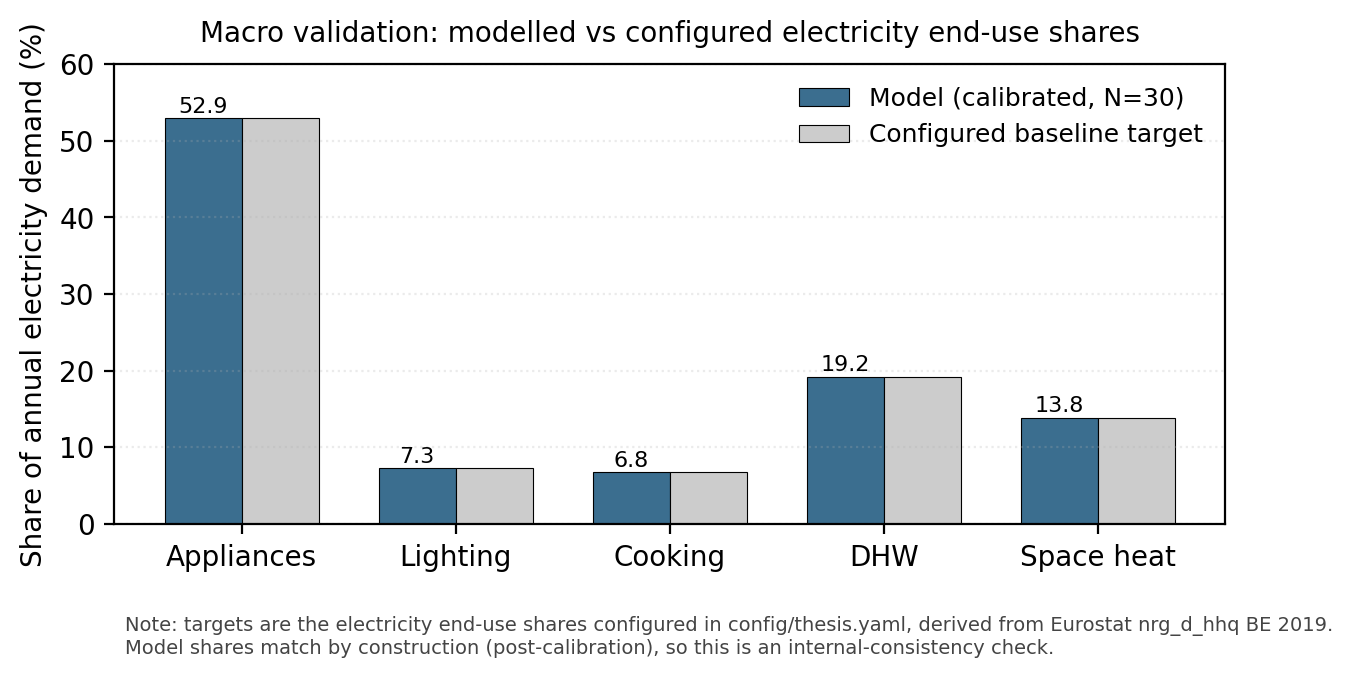
\includegraphics[width=\textwidth]{figures/macro_end_use_shares.png}
%   \caption{Macro validation: modelled cohort electricity end-use shares vs the configured baseline targets (derived from Eurostat \texttt{nrg\_d\_hhq} BE\,2019).}
%   \label{fig:macro_end_use_shares}
% \end{figure}
% Bars match by construction because the model rescales electricity to the configured end-use shares; the figure therefore reports calibration convergence, not external validation.

A full-horizon ($8760$-h) baseline-annual rerun under the thesis configuration, with the envelope calibration of \Cref{sec:modelv3} set to $0.80$ clears all three annual checks: calibrated electricity \SI{3500}{kWh}, useful space-heating thermal demand \SI{15162}{kWh}, and DHW thermal demand \SI{3000}{kWh}, each inside its configured Belgian range. The space-heating total is reported as a thermal baseline calibration, not as an independently validated envelope parameter (\Cref{sec:limitations}).


\subsection{Synthetic Validation}
\label{sec:syntheticValidation}
%%% Richardson / CREST for electricity realism
%%% Fischer et al. for thermal realism
%%% what each benchmark can and cannot support

The synthetic layer exercises the pipeline against a stochastic reference profile whose properties are themselves derived from a generative model rather than a measurement. Two runners cover this layer. The \textit{deterministic synthetic} runner generates a benchmark profile from the configured Belgian baseline bands and feeds the cohort engine through it, primarily as a regression test for the validation pipeline itself. The \emph{Richardson} runner compares the cohort's stochastic baseload structure against Richardson-style domestic profiles \cite{Richardson2010CRESTElectricity,Richardson2010_DomesticHighRes}, which are the canonical synthetic baseline for high-resolution residential electricity modelling. Both runners apply the variance, distribution, and temporal-structure metric families of \Cref{tab:validation_metrics}. The diversity factor computed by \texttt{compute\_diversity\_factor} is the ratio of the sum of individual peaks to the aggregate cohort peak, and is the most sensitive single metric here because it is determined by whether the cohort produces realistic non-coincidence of peak demand.

% % --- fig:synthetic_load_duration_curve ---
% \begin{figure}[ht]
%   \centering
%   \includegraphics[width=0.85\textwidth]
%     {figures/synthetic_load_duration_curve.png}
%   \caption{Synthetic validation: modelled versus synthetic reference load-duration curve.}
%   \label{fig:synthetic_load_duration_curve}
% \end{figure}


% % --- fig:diversity_by_household_count ---
% \begin{figure}[ht]
%   \centering
%   \includegraphics[width=\textwidth]
%     {figures/diversity_by_household_count.png}
%   \caption{Synthetic validation: diversity factor as a function of cohort size, demonstrating the expected convergence toward a stable peak-coincidence value as $N$ grows.}
%   \label{fig:diversity_by_household_count}
% \end{figure}


\subsection{Smart-Meter Validation}
\label{sec:smartMeterValidation}
%%% aggregate realism
%%% distributional realism
%%% UK measured data as external realism check; we don't have anything to pose as "Belgian ground truth"

The smart-meter layer is the only one that compares the cohort directly to observed Belgian residential meter data. It has two sub-tracks because the two available datasets are fundamentally different in cardinality and resolution.

\subsubsection*{Aggregate Fluvius}
The Flemish DSO Fluvius publishes representative \SI{15}{min} residential profiles disaggregated by heat-pump, EV, and PV indicators \cite{Fluvius2024OpenData}. The runner loads the relevant equipment combinations, aggregates them to a representative profile, time-aligns the model cohort to the Brussels timezone, and computes the mean-accuracy, temporal-structure, variance, and distribution metrics of \Cref{tab:validation_metrics}. Acceptance follows the ASHRAE-style thresholds, with explicit external-verdict thresholds added on top (\texttt{CVRMSE\_absolute\_pct $\le 50$}, \texttt{annual\_energy\_error\_pct $\le 25$}, Pearson $\ge 0.5$, $|$peak-timing error$|$ $\le 6\,$h).
% \newline The current persisted artefact reports a \texttt{weak\_failed\_external\_validation} verdict against these thresholds, meaning the aggregate profile is not yet aligned with the Fluvius representative profile. This is reported honestly rather than suppressed: it is the central open validation issue and is treated as such in \Cref{sec:limitations}\footnote{A Fluvius profile is a \emph{representative} category profile, not a measured feeder load, so the verdict supports aggregate profile plausibility rather than distribution-network feasibility.}.

\subsubsection*{High-frequency case study}
The KU\,Leuven three-house dataset \cite{KULeuven3House} provides high-frequency residential meter data for three Belgian dwellings of contrasting EPC and equipment (\Cref{tab:kul_houses}). The runner runs the model in a per-house mode and computes event-realism diagnostics: $24$-hour overlay segments, ramp-rate histograms, and spike-comparison plots. With $N=3$ this layer cannot support a statistical claim; it functions as a high-frequency \emph{event-realism} check, complementary to the aggregate Fluvius layer.

% % --- fig:fluvius_mean_daily_overlay ---
% \begin{figure}[ht]
%   \centering
%   \includegraphics[width=\textwidth]
%     {figures/fluvius_mean_daily_overlay.png}
%   \caption{Smart-meter validation: cohort versus Fluvius representative profile, full $2023$ hourly overlay.}
%   \label{fig:fluvius_mean_daily_overlay}
% \end{figure}


% % --- fig:kuleuven_house1_24h ---
% \begin{figure}[ht]
%   \centering
%   \includegraphics[width=\textwidth]
%     {figures/kuleuven_house1_24h.png}
%   \caption{Smart-meter validation: representative 24-hour segment for KU\,Leuven \texttt{house\_1}, showing event-realism on the high-frequency side.}
%   \label{fig:kuleuven_house1_24h}
% \end{figure}


\subsection{Technology Validation}
\label{sec:technologyValidation}

PV and EV are the two new technology layers added in \hyperref[sec:modelv3]{model v3}. Each is validated against its own references, independently of the household-cohort comparison above.

\subsubsection*{PV triangle}
The PV runner cross-checks the PV submodel against three references. The first leg compares the model's irradiance-to-PV conversion against a $\SI{1}{kWp}$ PVGIS hourly export \cite{Huld2012PVGIS}; the second leg compares the model's daily capacity factor against the Elia ODS032 country-level PV generation series \cite{Elia2024PVODS032}; the third leg compares the cohort PV net-load against the Fluvius residential \emph{with-PV} signature \cite{Fluvius2024OpenData}. The persisted artefact reports a Pearson correlation of $0.998$ on the PVGIS leg ($\text{hourly CF MAE} = 0.011$), a daily-CF correlation of $0.976$ on the Elia leg, and a monthly mean-absolute capacity-factor error of about $25\,\%$, which is consistent with single-chain modelling against country aggregate PV \cite{Pfeifroth2018SARAH}.

% % --- fig:pv_pvgis_reference ---
% \begin{figure}[ht]
%   \centering
%   \includegraphics[width=\textwidth]
%     {figures/pv_pvgis_reference.png}
%   \caption{PV validation: physical-reference leg of the model's irradiance-to-PV conversion against the PVGIS hourly \SI{1}{kWp} export, with hourly Pearson $r = 0.998$.}
%   \label{fig:pv_pvgis_reference}
% \end{figure}


% % --- fig:pv_elia_capacity_factor ---
% \begin{figure}[ht]
%   \centering
%   \includegraphics[width=\textwidth]
%     {figures/pv_elia_capacity_factor.png}
%   \caption{PV validation: Elia ODS032 Belgian country-level PV capacity factor for $2023$, with daily capacity-factor correlation $\approx 0.976$.}
%   \label{fig:pv_elia_capacity_factor}
% \end{figure}

\subsubsection*{EV}
The EV runner compares the model EV home-charging profile against the Fluvius \emph{EV signature} constructed as the difference between the EV-no-PV and no-EV-no-PV representative profiles. The persisted artefact reports a mean-daily Pearson correlation of $0.946$, a peak-hour match at \texttt{01:00}, and an annual-energy gap of $-43\,\%$ against the Fluvius positive EV increment ($\SI{2626}{kWh}$ per reference meter), which closes to $-1\,\%$ under a sensitivity that rescales annual home-charging to $\SI{2600}{kWh}$ while preserving the model timing shape. This is treated as a category-profile signature check, not as a session-level charging validation \cite{Fluvius2024OpenData}.

% % --- fig:ev_signature ---
% \begin{figure}[ht]
%   \centering
%   \includegraphics[width=\textwidth]
%     {figures/ev_fluvius_signature.png}
%   \caption{EV technology validation: mean-daily overlay of the Fluvius residential EV signature versus the model EV home-charging profile.}
%   \label{fig:ev_signature}
% \end{figure}


\subsection{Validation Summary}
\label{sec:validationSummary}

\Cref{tab:validation_summary} consolidates what each layer supports, the reference dataset, and the most informative metric family. Two honest constraints follow from this table. First, the macro layer is internal-consistency, not external validation, because the calibration target is also the comparison target. Second, the aggregate Fluvius layer is the strictest external profile-shape test and is therefore treated as the central validation stress test in \Cref{ch:results}; until that comparison is evaluated, smart-meter realism is interpreted through both the aggregate Fluvius profile and the KU\,Leuven event-realism case study.

\begin{table}[ht]
  \centering
  \footnotesize
  \caption{Validation matrix. Each row maps one layer to its reference dataset, the family of metrics evaluated, and what the layer does and does not support.}
  \label{tab:validation_summary}
  \begin{tabular}{@{}p{0.18\linewidth} p{0.22\linewidth}
                   p{0.18\linewidth} p{0.32\linewidth}@{}}
    \toprule
    \textbf{Layer} & \textbf{Reference} &
      \textbf{Primary metric} & \textbf{Supports / does not support} \\
    \midrule
    Macro
      & Eurostat \texttt{nrg\_d\_hhq} BE shares
        \cite{eurostat_disaggregated_nodate}
      & end-use share error
      & supports annual calibration convergence; does not support
        external validation \\
    Synthetic / Richardson
      & Richardson-style stochastic profile
        \cite{Richardson2010CRESTElectricity}
      & variance, $r$, diversity factor
      & supports stochastic structure plausibility; does not
        constrain absolute magnitudes \\
    Smart-meter aggregate
      & Fluvius representative profiles
        \cite{Fluvius2024OpenData}
      & CVRMSE, peak-timing, Anderson--Darling
      & currently fails the external verdict; treated as open issue \\
    Smart-meter high-frequency
      & KU\,Leuven three-house dataset
        \cite{KULeuven3House}
      & ramp histogram, peak MAE
      & supports event-realism qualitatively; $N=3$ precludes a
        statistical claim \\
    PV triangle
      & PVGIS \cite{Huld2012PVGIS}, Elia ODS032
        \cite{Elia2024PVODS032}
      & hourly $r$, daily CF
      & supports PV submodel; does not validate cohort
        self-consumption \\
    EV
      & Fluvius EV signature \cite{Fluvius2024OpenData}
      & daily $r$, peak-hour match
      & supports EV signature shape; does not validate session-level
        charging \\
    \bottomrule
  \end{tabular}
\end{table}



\mode<all> % do not remove
